\documentclass[11pt,a4paper]{article}

\usepackage[T1]{fontenc}
\usepackage[utf8]{inputenc}
\usepackage[english]{babel}
\usepackage[a4paper,margin=2.4cm]{geometry}
\usepackage{amsmath,amssymb}
\usepackage{booktabs}
\usepackage{longtable}
\usepackage{array}
\usepackage{enumitem}
\usepackage{microtype}
\usepackage{tikz}
\usetikzlibrary{positioning,arrows.meta}
\usepackage[hidelinks]{hyperref}

\newcolumntype{L}[1]{>{\raggedright\arraybackslash}p{#1}}
\newcommand{\mpart}[1]{\smallskip\noindent\textbf{#1}\ \ignorespaces}
\setlist[itemize]{noitemsep,topsep=3pt,leftmargin=*}
\setlist[enumerate]{noitemsep,topsep=3pt,leftmargin=*}
\setlength{\parskip}{2pt}
\renewcommand{\arraystretch}{1.15}

\newcommand{\prox}{\operatorname{prox}}
\newcommand{\lse}{\operatorname{lse}}
\newcommand{\dom}{\operatorname{dom}}

\title{\textbf{A Reading Plan on the Mathematical Foundations}\\[3pt]
\large MMC007 --- Optimization}
\author{MSc in Mathematical and Computational Modeling\\
IMCA --- Faculty of Sciences, Universidad Nacional de Ingenier\'ia}
\date{Semester 2026--2}

\begin{document}

\maketitle

\section{Objective and scope}

The MMC007 syllabus states the course as three lists of methods. \emph{Convex
programming}: properties of convex sets and convex functions, conjugacy and the
subdifferential, duality and the Lagrangian, the subgradient method, the proximal method.
\emph{Linear programming}: applications, properties, the simplex method in its primal and
dual forms, sensitivity analysis, interior point methods, and integer programming by branch
and bound, Benders decomposition and column generation. \emph{Differentiable programming}:
optimality conditions, descent algorithms, line search, the gradient method, projected
gradient, conjugate gradient, Newton, quasi-Newton, Frank--Wolfe, Gauss--Seidel, Uzawa's
algorithm, the augmented Lagrangian, trust regions, interior point methods.

Read in that order, the course is a catalogue of some thirty procedures divided into three
compartments that appear to share nothing. This plan covers the same content but reorders it
by the \emph{mathematical structure that makes each algorithm work}, so that every method
arrives as the consequence of a theorem rather than as a recipe, and so that the three
compartments are revealed to be one subject. Four cores carry the whole syllabus:

\begin{enumerate}
\item \textbf{Separation.} A point not in a closed convex set can be strictly separated from
it by a hyperplane. This single geometric fact produces Farkas' lemma, the duality theorem of
linear programming, the Karush--Kuhn--Tucker conditions, and Fenchel duality. The plan's
central claim is that these are not four theorems but one.
\item \textbf{Conjugacy and the subdifferential.} The Fenchel conjugate and the
subdifferential turn nondifferentiable convex functions into objects with a calculus, and
they generate the proximal operator, which is what every algorithm in the nonsmooth part of
the course actually computes.
\item \textbf{Smoothness and strong convexity.} Two inequalities --- the descent lemma above
and the strong-convexity bound below --- are the source of every convergence rate stated in
the course. Once they are proved, the rates of the gradient method, the projected gradient,
Frank--Wolfe, the proximal gradient, and their accelerated forms are corollaries obtained by
substitution.
\item \textbf{Polyhedral geometry.} Faces, extreme points and the Minkowski--Weyl theorem
explain why linear programs have vertex solutions, why the simplex method is a finite
algorithm at all, and --- through total unimodularity --- when the integrality constraint of
an integer program is free.
\end{enumerate}

\subsection*{Three structural decisions}

\mpart{No block of prerequisites.} There is no introductory module on convex analysis, linear
algebra and topology. Each module develops exactly the mathematics it needs, at the point
where it is needed, following the expository method of Zhao's \emph{Mathematical Foundations
of Reinforcement Learning}: state the idea and the algorithm first, then descend into why it
works. The projection theorem therefore appears inside separation, conjugacy inside the
proximal operator, the calculus of tangent cones inside optimality conditions, Krylov
subspaces inside the conjugate gradient method, and self-concordance inside interior point
methods. Every module lists its \emph{foundation developed here} explicitly, so nothing is
silently assumed.

\mpart{Every module has a programming section.} Each module closes with a proof-of-concept
implementation whose purpose is to \emph{verify the theorem numerically}, not to produce a
usable solver. The rule throughout is: implement in NumPy from scratch, and use
\texttt{scipy.optimize}, \texttt{cvxpy} or an integer programming package only as a
correctness oracle to compare against. Each proof of concept states a validation check: a
number that must come out right if the mathematics was understood.

\mpart{Every module names its reinforcement-learning instantiation.} The stated purpose of
taking this course to a high standard is to be able to develop reinforcement learning
algorithms afterwards. Optimization is not a tool that reinforcement learning happens to use;
the central objects of reinforcement learning \emph{are} optimization objects. The softmax
policy is the gradient of a conjugate function (M3); the constrained Markov decision process
is a Lagrangian saddle point (M4); trust region policy optimization is a trust region
subproblem solved by conjugate gradients on Hessian-vector products (M6, M7); the natural
policy gradient is mirror descent with the Kullback--Leibler Bregman divergence (M9); the
discounted Markov decision process is a linear program whose dual variable is the occupancy
measure and whose complementary slackness condition is the greedy policy (M11). Each module
states its instantiation in one or two sentences. Reinforcement learning is never a primary
reading; it is only the object the theorem is applied to. Module M15 is the exception, and it
is explicitly an extension.

\subsection*{Effort}

Fifteen modules, approximately 123 hours of reading, written proofs and programming, of which
113 hours are the fourteen core modules and 10 the extension. Note that the 48 hours recorded
for MMC007 in the study plan are \emph{contact} hours; this plan is the self-study that
accompanies them, and works out to roughly seven and a half hours per week over a sixteen-week
semester.

This is heavier than proportional. The MMC201 plan allots 93 hours against 64 contact hours;
this one allots 123 against 48. Two reasons. First, MMC007 states three programming
paradigms where MMC201 states one family of models, and each paradigm carries its own
algorithms and its own convergence theory. Second, the reinforcement-learning objective
requires that the convex-analytic and duality material be understood at the level of proof
rather than of statement, since that is the material one manipulates when designing an
algorithm rather than applying one. A reader who only needs to pass the course can drop M15
and read M13 and M14 for statements rather than proofs, which returns the plan to about 90
hours.

\subsection*{Relation to the syllabus}

Modules M1--M14 cover the syllabus in full, with no orphan topic: every topic named in
the contents appears in exactly one module's \emph{foundation developed here}. Module M15
(stochastic approximation) is an \emph{extension}: it is not listed in the MMC007 contents,
and is included because it is what converts the course into a working basis for
reinforcement learning algorithm design. It can be omitted without breaking anything else.

Two of the syllabus items appear twice in the official contents and once here. ``Interior
point methods'' is listed under linear programming and again under differentiable
programming; both occurrences are M13, since the barrier method for a linear program and the
barrier method for a smooth convex program differ only in which self-concordant function is
used. ``Optimality conditions'' appears under differentiable programming but is inseparable
from ``duality and the Lagrangian notion'' under convex programming; both are M4.

A terminological warning, since the syllabus uses the word ``duality'' for what looks like
three unrelated subjects. \emph{Lagrangian duality} (convex programming), \emph{linear
programming duality} (the simplex method's dual), and \emph{conjugate duality} (Fenchel
conjugation) are stated in three different places in the contents. The claim organizing this
plan is that they are one theorem stated three times: conjugate duality is proved in M3,
Lagrangian duality in M4, and linear programming duality is obtained in M11 as the special
case in which the constraint qualification is automatic. A reader who treats them as three
subjects will learn the course three times.

\clearpage

\section{Dependencies between modules}

The plan is not a linear sequence. Table~\ref{tab:dep} fixes the dependencies and
Figure~\ref{fig:dag} draws them. The rule is that a module may be started only when every
module in its \emph{Requires} column has been completed, meaning both its written checkpoint
and its programming validation check have been passed.

\begin{table}[htbp]
\centering
\small
\caption{Module dependencies.}
\label{tab:dep}
\begin{tabular}{@{}l L{6.4cm} L{2.6cm} L{3.2cm}@{}}
\toprule
\textbf{Mod.} & \textbf{Title} & \textbf{Requires} & \textbf{Enables} \\
\midrule
M1  & Convex sets, separation and Farkas                     & ---            & M2, M4 \\
M2  & Convex functions, smoothness and strong convexity      & M1             & M3, M5 \\
M3  & Conjugacy, subdifferential and the proximal operator   & M2             & M4, M9 \\
M4  & Optimality conditions and Lagrangian duality           & M1, M3         & M8, M10, M11 \\
M5  & Line search and the gradient method                    & M2             & M6, M8, M9 \\
M6  & Newton, quasi-Newton and trust regions                 & M5             & M7, M13 \\
M7  & Conjugate gradient and matrix-free optimization        & M6             & M15 \\
M8  & Projected gradient, Frank--Wolfe, Gauss--Seidel        & M4, M5         & M14 \\
M9  & Subgradient, proximal and mirror descent               & M3, M5         & M10, M15 \\
M10 & Augmented Lagrangian, Uzawa and splitting              & M4, M9         & M14 \\
M11 & Polyhedra, linear programming and LP duality           & M4             & M12, M13, M15 \\
M12 & The simplex method and sensitivity analysis            & M11            & M14 \\
M13 & Interior point methods and self-concordance            & M6, M11        & --- \\
M14 & Branch and bound, Benders, column generation           & M8, M10, M12   & --- \\
M15 & Stochastic approximation for RL (extension)            & M7, M9, M11    & --- \\
\bottomrule
\end{tabular}
\end{table}

Three observations about the graph:

\begin{itemize}
\item \textbf{M4 is the bottleneck.} Optimality conditions and Lagrangian duality
simultaneously require separation (M1) and conjugacy (M3). Without M4 nothing downstream can
be motivated: the projected gradient of M8 is stationarity stated in terms of the normal
cone, the multiplier update of M10 is a step on the dual function, the duality theorem of M11
is the polyhedral special case, and the central path of M13 is the perturbed KKT system.
Every one of these is a restatement of M4 in a particular setting, and a reader who leaves M4
half-understood will experience them as four unrelated tricks.

\item \textbf{There are two independent branches.} After M4 the branch M5--M10 (algorithms
for continuous problems, smooth then nonsmooth) and the branch M11--M13 (polyhedral geometry,
the simplex method, interior point methods) share no dependency except M6, which M13 needs
for Newton's method. They may be read in either relative order, or in parallel by two
readers. For a thesis pointing at reinforcement learning, run M5--M10 first: M9 is the module
that pays off most directly.

\item \textbf{The branches meet in the last three modules, and that is the point.} M14 needs
the decomposition ideas of M10 and the polyhedral bounds of M12 in the same argument, because
Benders decomposition is Lagrangian duality applied to a linear subproblem and column
generation is the same construction transposed. M15 needs the mirror step of M9, the
Krylov machinery of M7 and the linear programming formulation of M11 at once. If the two
branches still feel like separate subjects when M13 is reached, the reason is almost always
that M4 was read as a list of conditions rather than as a theorem about separation.
\end{itemize}

\begin{figure}[htbp]
\centering
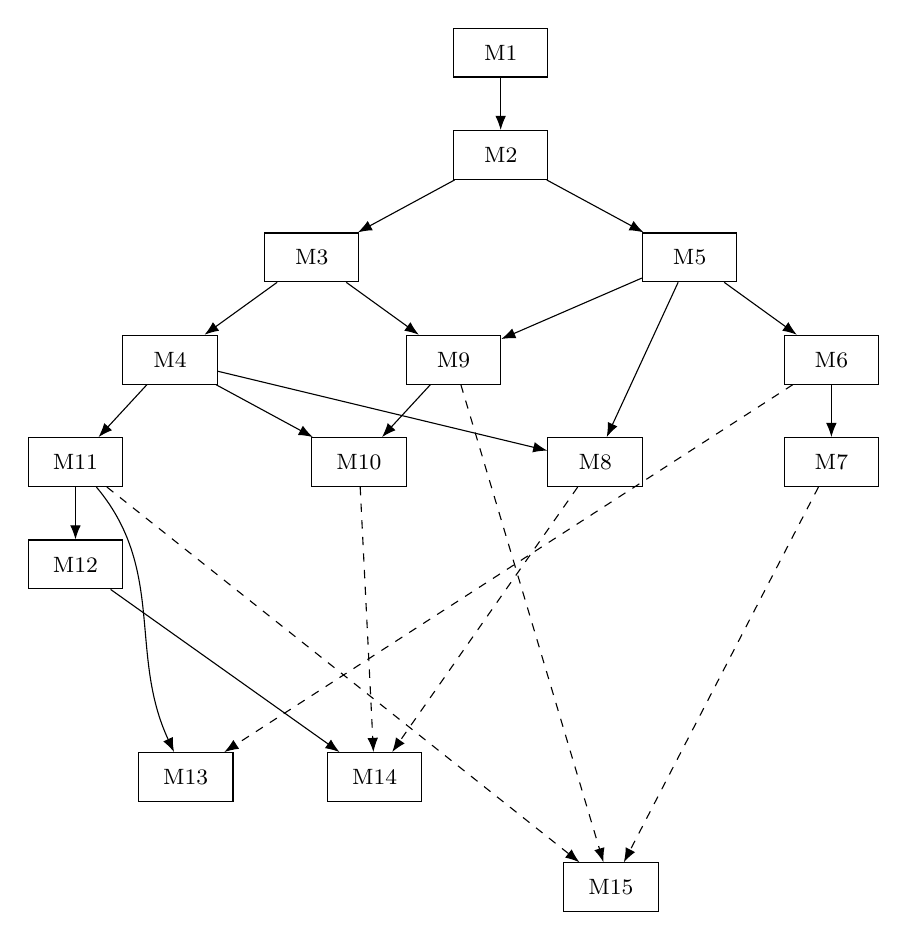
\begin{tikzpicture}[
  every node/.style={font=\footnotesize},
  mod/.style={draw, rectangle, minimum width=12mm, minimum height=6.2mm, inner sep=2pt},
  ar/.style={-{Latex[length=1.8mm]}, thin},
  cr/.style={-{Latex[length=1.8mm]}, thin, dashed}
]
\node[mod] (m1)  at (6.0,  0)    {M1};
\node[mod] (m2)  at (6.0, -1.3)  {M2};
\node[mod] (m3)  at (3.6, -2.6)  {M3};
\node[mod] (m5)  at (8.4, -2.6)  {M5};
\node[mod] (m4)  at (1.8, -3.9)  {M4};
\node[mod] (m9)  at (5.4, -3.9)  {M9};
\node[mod] (m6)  at (10.2,-3.9)  {M6};
\node[mod] (m11) at (0.6, -5.2)  {M11};
\node[mod] (m10) at (4.2, -5.2)  {M10};
\node[mod] (m8)  at (7.2, -5.2)  {M8};
\node[mod] (m7)  at (10.2,-5.2)  {M7};
\node[mod] (m12) at (0.6, -6.5)  {M12};
\node[mod] (m13) at (2.0, -9.2)  {M13};
\node[mod] (m14) at (4.4, -9.2)  {M14};
\node[mod] (m15) at (7.4, -10.6) {M15};

\draw[ar] (m1)  -- (m2);
\draw[ar] (m2)  -- (m3);
\draw[ar] (m2)  -- (m5);
\draw[ar] (m3)  -- (m4);
\draw[ar] (m3)  -- (m9);
\draw[ar] (m5)  -- (m9);
\draw[ar] (m5)  -- (m6);
\draw[ar] (m5)  -- (m8);
\draw[ar] (m4)  -- (m11);
\draw[ar] (m4)  -- (m10);
\draw[ar] (m4)  -- (m8);
\draw[ar] (m9)  -- (m10);
\draw[ar] (m6)  -- (m7);
\draw[ar] (m11) -- (m12);
\draw[ar] (m11) to[out=-50,in=115] (m13);
\draw[ar] (m12) -- (m14);

\draw[cr] (m6)  -- (m13);
\draw[cr] (m8)  -- (m14);
\draw[cr] (m10) -- (m14);
\draw[cr] (m7)  -- (m15);
\draw[cr] (m9)  -- (m15);
\draw[cr] (m11) -- (m15);
\end{tikzpicture}
\caption{Dependency graph. An arrow $A \rightarrow B$ means $A$ must be completed before
starting $B$. For legibility the figure shows the transitive reduction: edges implied by
composition, such as M1 $\rightarrow$ M4 via M2 and M3, are omitted. Table~\ref{tab:dep}
lists the full requirements. Dashed arrows are the requirements that cross from one branch to
the other; they occur only into M13, M14 and M15, which is exactly where the continuous and
the polyhedral halves of the course meet.}
\label{fig:dag}
\end{figure}

The \textbf{critical path} is M1 $\to$ M2 $\to$ M3 $\to$ M4 $\to$ M11 $\to$ M12 $\to$ M14.
No reordering of these seven modules is possible. The longest chain in the continuous branch,
M1 $\to$ M2 $\to$ M5 $\to$ M6 $\to$ M7 $\to$ M15, is one module shorter and can be run
concurrently with it.

\clearpage

\section{Reading sequence}

Table~\ref{tab:seq} gives the order of study. The primary readings are the nine texts of the
MMC007 syllabus. The foundation readings are drawn from Section~\ref{sec:bib} and are the
reason the plan can claim to explain \emph{why} the algorithms work rather than only what
they compute; short labels such as \emph{Rockafellar} refer to the bibliography. Where a
syllabus text is not organized by numbered chapters that can be cited safely, the cell names
the relevant part in words.

\begin{longtable}{@{}L{0.9cm} L{3.3cm} L{4.1cm} L{4.7cm} L{1.2cm}@{}}
\caption{Reading sequence for MMC007.}\label{tab:seq}\\
\toprule
\textbf{Mod.} & \textbf{Topic} & \textbf{Primary reading} & \textbf{Foundation reading} & \textbf{Hours} \\
\midrule
\endfirsthead
\multicolumn{5}{@{}l}{\small\itshape Table \thetable{} (continued)}\\
\toprule
\textbf{Mod.} & \textbf{Topic} & \textbf{Primary reading} & \textbf{Foundation reading} & \textbf{Hours} \\
\midrule
\endhead
\midrule
\multicolumn{5}{r@{}}{\small\itshape continued on next page}\\
\endfoot
\bottomrule
\endlastfoot

M1 & Convex sets, separation and Farkas
   & Crouzeix--Oca\~na (convex sets, separation); Izmailov--Solodov (convex analysis); Bertsekas NLP App.~B
   & Rockafellar \S 2--3, 11, 18--19; Hiriart-Urruty--Lemar\'echal~A; Boyd--Vandenberghe ch.~2; Farkas (1902)
   & 7 \\

M2 & Convex functions, smoothness and strong convexity
   & Crouzeix--Oca\~na (convex functions); Bertsekas NLP \S 1.1; Nocedal--Wright ch.~2
   & Boyd--Vandenberghe ch.~3; Hiriart-Urruty--Lemar\'echal~B; Beck FOM ch.~5; Nesterov \S 2.1
   & 6 \\

M3 & Conjugacy, subdifferential and prox
   & Crouzeix--Oca\~na (conjugacy, subdifferential); Izmailov--Solodov (convex analysis and duality)
   & Rockafellar \S 12, 16, 23--25; H-U--Lemar\'echal~D--E; Beck FOM ch.~3--4, 6; Bauschke--Combettes ch.~12, 24; Moreau (1965)
   & 9 \\

M4 & Optimality conditions and Lagrangian duality
   & Bertsekas NLP ch.~3 and 5; Izmailov--Solodov (optimality conditions); Luenberger ch.~11
   & Rockafellar \S 27--30; Boyd--Vandenberghe ch.~4--5; Nocedal--Wright ch.~12; Kuhn--Tucker (1951); Sion (1958)
   & 9 \\

M5 & Line search and the gradient method
   & Nocedal--Wright ch.~3; Bertsekas NLP \S 1.2; Luenberger ch.~7--8
   & Nesterov ch.~1--2; Beck FOM ch.~10; Polyak (1963); Nesterov (1983)
   & 8 \\

M6 & Newton, quasi-Newton and trust regions
   & Nocedal--Wright ch.~4 and 6; Bertsekas NLP \S 1.3--1.4; Luenberger ch.~10
   & Conn--Gould--Toint ch.~6--7; Dennis--Mor\'e (1974); Powell (1970); Steihaug (1983)
   & 9 \\

M7 & Conjugate gradient and matrix-free optimization
   & Nocedal--Wright ch.~5 and 7; Luenberger ch.~9
   & Trefethen--Bau lect.~38; Saad ch.~6; Golub--Van Loan \S 11.3; Hestenes--Stiefel (1952); Fletcher--Reeves (1964)
   & 7 \\

M8 & Projected gradient, Frank--Wolfe, Gauss--Seidel
   & Bertsekas NLP ch.~2; Nocedal--Wright \S 16.7
   & Beck FOM ch.~9--11, 13--14; Frank--Wolfe (1956); Jaggi (2013); Powell (1973); Nesterov (2012)
   & 7 \\

M9 & Subgradient, proximal and mirror descent
   & Bertsekas, \emph{Convex Optimization Algorithms} ch.~3; Izmailov--Solodov (nonsmooth methods)
   & Beck FOM ch.~8--10, 12; Nesterov ch.~3; Nemirovski--Yudin; Beck--Teboulle (2003, 2009); Rockafellar (1976b)
   & 9 \\

M10 & Augmented Lagrangian, Uzawa and splitting
   & Bertsekas NLP ch.~4; Nocedal--Wright ch.~17
   & Bertsekas, \emph{Constrained Optimization and Lagrange Multiplier Methods} ch.~2--3; Uzawa (1958); Rockafellar (1976a); Boyd et al.\ (2011)
   & 8 \\

M11 & Polyhedra, linear programming and LP duality
   & Chv\'atal ch.~1--2, 5; Bertsimas--Tsitsiklis ch.~2 and 4; Dantzig--Thapa vol.~1; Wolsey ch.~1
   & Schrijver \S 7--8, 19; Ziegler ch.~1--2; Manne (1960)
   & 8 \\

M12 & The simplex method and sensitivity analysis
   & Chv\'atal ch.~2--4 and 7 and the sensitivity chapter; Bertsimas--Tsitsiklis ch.~3 and 5; Dantzig--Thapa vol.~1
   & Schrijver \S 11; Golub--Van Loan \S 3.2 (LU); Bland (1977); Klee--Minty (1972)
   & 9 \\

M13 & Interior point methods and self-concordance
   & Bertsimas--Tsitsiklis ch.~9; Nocedal--Wright ch.~14 and 19; Luenberger ch.~5
   & Renegar ch.~1--2; S.~Wright ch.~1--2, 5; Nesterov ch.~5; Nesterov--Nemirovskii; Karmarkar (1984); Mehrotra (1992)
   & 8 \\

M14 & Branch and bound, Benders, column generation
   & Wolsey ch.~2, 7--8, 10--11; Nemhauser--Wolsey (polyhedral theory, general algorithms); Bertsimas--Tsitsiklis ch.~6, 10--11
   & Conforti--Cornu\'ejols--Zambelli ch.~3--5, 8--9; Schrijver \S 23; Land--Doig (1960); Benders (1962); Dantzig--Wolfe (1960); Gilmore--Gomory (1961)
   & 9 \\

M15 & Stochastic approximation for RL (extension)
   & --- (no MMC007 text)
   & Borkar ch.~2, 6; Puterman \S 6.9; Bertsekas--Tsitsiklis NDP ch.~4; Agarwal et al.\ (policy gradient); Robbins--Monro (1951); Tsitsiklis--Van Roy (1997); Kakade (2001)
   & 10 \\
\midrule
   &  &  & \textbf{Total} & \textbf{123} \\
\end{longtable}

\clearpage

\section{The programming track}

Every module has a proof-of-concept implementation. Its purpose is diagnostic: it must
reproduce, as a number, something the theorem predicts. If the number does not come out, the
mathematics was not understood, and the module is not finished.

\mpart{Rules.} Implement in Python with NumPy and SciPy only. Do not call a library routine
for the object under study: write the solver. Established libraries
(\texttt{scipy.optimize} with the HiGHS backend, \texttt{cvxpy}, \texttt{python-mip}) are
permitted only as an oracle, to confirm that your implementation agrees with a trusted one.
Fix random seeds and report tolerances; a validation check without a tolerance is not a
check. Keep each module in its own notebook or script, since several later modules reuse
earlier code: M13 reuses the Newton step of M6 and the Krylov solver of M7; M14 reuses the
revised simplex of M12 for its warm starts and the cut generation of M10; M15 reuses the
mirror step of M9 and the Markov decision process of M11.

\mpart{A note on scale.} Every problem in this track is small on purpose --- a few dozen
variables, a few hundred iterations. The point is never performance. A validation check that
requires a large instance to become visible has been designed wrongly, and should be replaced
by one that can be checked against an analytic answer.

\begin{longtable}{@{}L{0.9cm} L{6.2cm} L{7.3cm}@{}}
\caption{Proof-of-concept implementations and their validation checks.}\label{tab:poc}\\
\toprule
\textbf{Mod.} & \textbf{Implement} & \textbf{Validation check} \\
\midrule
\endfirsthead
\multicolumn{3}{@{}l}{\small\itshape Table \thetable{} (continued)}\\
\toprule
\textbf{Mod.} & \textbf{Implement} & \textbf{Validation check} \\
\midrule
\endhead
\midrule
\multicolumn{3}{r@{}}{\small\itshape continued on next page}\\
\endfoot
\bottomrule
\endlastfoot

M1 & Euclidean projection onto the probability simplex, onto a halfspace and onto the
     second-order cone, each from scratch; a routine that produces the Farkas certificate of
     an infeasible system
   & $\langle x-P_C x,\ y-P_C x\rangle \le 0$ for every sampled $y \in C$, to $10^{-12}$;
     $\|P_C x - P_C z\| \le \|x-z\|$ on random pairs; the returned Farkas vector $y$ satisfies
     $A^\top y \ge 0$, $b^\top y < 0$ exactly, and no feasible $x$ is found by the oracle \\

M2 & Numerical estimation of $L$ and $\mu$ for a regularized logistic objective from the
     extreme Hessian eigenvalues; evaluation of both bounds at random pairs
   & The descent lemma and the strong-convexity bound hold at every sampled pair, and both
     become equalities to $10^{-8}$ along the corresponding extreme eigendirection of a
     quadratic, which is what makes $L$ and $\mu$ the correct constants and not merely valid
     ones \\

M3 & Conjugates and proximal operators of $\|\cdot\|_1$, $\|\cdot\|_2$, the indicator of the
     simplex and negative entropy; the Moreau envelope; the log-sum-exp function
   & Moreau decomposition $x=\prox_f(x)+\prox_{f^*}(x)$ to machine precision; the numerical
     $\nabla$ of the Moreau envelope equals $(x-\prox_{\lambda f}(x))/\lambda$;
     $\nabla \lse$ equals the softmax equals the argmax of the entropy-regularized linear
     program over the simplex, all three to $10^{-10}$ \\

M4 & KKT residuals for random convex quadratic programs with linear constraints; the optimal
     value as a function of a perturbed right-hand side; one problem violating MFCQ
   & Stationarity, feasibility and complementarity residuals below $10^{-9}$ at the oracle
     solution; the multiplier $\lambda^\star$ matches the finite-difference derivative of
     $v(b)$ to $O(h)$; on the MFCQ-violating problem no multiplier exists, verified by the
     infeasibility of the KKT system \\

M5 & Gradient descent with exact, Armijo and Wolfe line searches on quadratics of prescribed
     condition number, and Nesterov's accelerated method on the same
   & The measured contraction factor matches $(\kappa-1)/(\kappa+1)$ for exact line search
     and $1-\mu/L$ for the constant step, within 5\%; the accelerated method matches
     $O(1/k^2)$; on Nesterov's worst-case function no first-order method in the run beats the
     lower bound at any $k$ \\

M6 & BFGS and L-BFGS with a Wolfe line search from scratch; a trust-region method with both
     the dogleg and the Steihaug--CG subproblem solver
   & The secant equation holds and $B_k \succ 0$ is preserved at every accepted step; the
     Dennis--Mor\'e ratio $\|(B_k-\nabla^2 f)p_k\|/\|p_k\| \to 0$ exactly on the runs that
     converge superlinearly and not on the others; the trust-region step never exceeds the
     radius and the predicted-to-actual reduction ratio governs the radius as specified \\

M7 & Linear CG from scratch; nonlinear CG (Fletcher--Reeves and Polak--Ribi\`ere$+$); a
     truncated Newton--CG that never forms the Hessian
   & Directions are $A$-orthogonal to $10^{-10}$ and the method terminates in at most $n$
     steps in exact arithmetic; the error in the $A$-norm decays at the
     $2((\sqrt\kappa-1)/(\sqrt\kappa+1))^k$ rate; Newton--CG reproduces the exact Newton step
     when the inner tolerance is driven to zero, using only Hessian-vector products \\

M8 & Projected gradient and Frank--Wolfe on the same simplex-constrained problem; cyclic
     block coordinate descent, run also on Powell's example
   & The Frank--Wolfe gap upper-bounds the true suboptimality at every iterate; Frank--Wolfe
     shows $O(1/k)$ and does \emph{not} accelerate under any of the standard step rules,
     while projected gradient does; the gradient mapping vanishes exactly at the projected
     fixed point; the cyclic scheme on Powell's function cycles without converging \\

M9 & Subgradient descent with $c/\sqrt{k}$ and Polyak steps; ISTA and FISTA; mirror descent
     on the simplex with the entropic Bregman divergence
   & Measured rates match $O(1/\sqrt k)$, $O(1/k)$ and $O(1/k^2)$ respectively; the objective
     is \emph{not} monotone under the subgradient method, which is the point; the mirror
     iterate equals the closed-form exponentiated-gradient update to $10^{-12}$; the iterates
     are Fej\'er monotone with respect to the solution set for the proximal point method \\

M10 & Uzawa, the quadratic penalty method, the augmented Lagrangian and ADMM on the same
      equality-constrained convex quadratic program
    & Uzawa converges for every step below the bound $2\mu/\|A\|^2$ predicted by the M3
      duality and diverges just above it; the augmented Lagrangian multiplier sequence equals
      the proximal-point sequence on the dual to $10^{-10}$; the penalty method's Hessian
      condition number grows like the penalty parameter while the augmented Lagrangian's does
      not \\

M11 & Vertex enumeration for a small polytope from both its H- and V-representations; a
      small discounted Markov decision process written as a linear program, solved in primal
      and dual form
    & The two representations generate the same set, which is Minkowski--Weyl tested
      directly; every enumerated vertex is a basic feasible solution and conversely; the dual
      optimum equals the discounted occupancy measure of the optimal policy computed
      independently by simulation, and complementary slackness recovers the greedy policy
      exactly \\

M12 & The revised simplex with Bland's rule and an LU basis factorization; the dual simplex;
      sensitivity ranging of $c$ and $b$; the Klee--Minty cube
    & Agreement with \texttt{linprog} on optimal value to $10^{-9}$ and on the optimal basis;
      Bland's rule terminates on a deliberately cycling instance where Dantzig's rule does
      not; the ranges are confirmed by re-solving at their endpoints; the pivot count on
      Klee--Minty is exactly $2^n-1$ \\

M13 & A primal--dual path-following method for linear programs from scratch, with Mehrotra's
      predictor--corrector as a variant
    & The duality gap equals $n\mu$ at every iterate to $10^{-10}$; the iterates stay in the
      prescribed neighbourhood of the central path; the iteration count to fixed accuracy
      grows like $\sqrt n$ over a sweep of problem sizes, not like $n$; the Newton decrement
      certifies the stopping accuracy it claims \\

M14 & Branch and bound over the M12 simplex with dual-simplex warm starts; Gomory cuts;
      Benders decomposition on a two-stage problem; column generation for cutting stock
    & The branch-and-bound optimum matches the oracle and the LP bound at every node is a
      valid lower bound; every Benders cut is valid at the incumbent and the master bound
      increases monotonically to the true optimum; column generation terminates exactly when
      the pricing subproblem returns a nonnegative reduced cost, and its bound matches the
      LP relaxation of the full formulation \\

M15 & Robbins--Monro on a root-finding problem with a known answer; TD(0) on a small chain;
      an off-policy divergence example with linear features; REINFORCE on a two-state Markov
      decision process
    & The Robbins--Monro iterate converges under $\sum\alpha_k=\infty$, $\sum\alpha_k^2<\infty$
      and visibly fails when either is violated; TD(0) converges to
      $(I-\gamma P^\pi)^{-1}r^\pi$ with error decaying at the predicted rate; Baird's
      counterexample diverges, confirming where the contraction argument breaks; the
      REINFORCE gradient estimate is unbiased for the analytically computed policy gradient
      within Monte-Carlo error \\
\end{longtable}

\clearpage

\section{The modules}

Each module has six parts: the \emph{idea} as a practitioner would state it; the
\emph{foundation developed here}, meaning the mathematics introduced at this point because
this is where it is first needed; the \emph{key results} to be stated and proved; the
\emph{readings}; the \emph{proof of concept}; and a written \emph{checkpoint}, chosen so that
it is reused explicitly in a later module. Several modules add a paragraph saying \emph{why
the module sits where it does}, and each names the reinforcement-learning object its theorems
govern.

\subsection{M1. Convex sets, separation and Farkas' lemma}

\mpart{Idea.} Everything in this course is an assertion that some point is or is not in some
convex set, and every proof that a candidate solution is optimal --- or that no solution
exists --- consists of exhibiting a hyperplane. This module proves the one geometric theorem
that the rest of the course quotes.

\mpart{Foundation developed here.} Affine and convex hulls, Carath\'eodory's theorem, the
relative interior and why it is the right notion of interior for a set that may be
lower-dimensional; closedness of convex sets and when the sum of two closed convex sets fails
to be closed; the \emph{projection onto a closed convex set}: existence, uniqueness, the
variational characterization $\langle x - P_C x,\ y - P_C x\rangle \le 0$ for all $y \in C$,
and nonexpansiveness; separating and supporting hyperplane theorems in their proper and
strict forms; cones, polar and dual cones, the bipolar theorem; polyhedral cones and Farkas'
lemma with its equivalent forms (Gordan, Stiemke, Motzkin).

\mpart{Key results.}
\begin{enumerate}
\item \textbf{Projection theorem.} For $C$ closed convex and any $x$ there is a unique
$P_C x \in C$ minimizing $\|x - c\|$ over $c \in C$, characterized by the variational
inequality above, and $P_C$ is nonexpansive. This is the finite-dimensional Hilbert space
projection theorem; MMC201's M2 uses the same statement for a linear subspace, where the
inequality becomes the equality $y - \hat y \perp S$.
\item \textbf{Separation.} If $x \notin C$ with $C$ closed convex, there is $a \ne 0$ and
$\alpha$ with $\langle a, x\rangle > \alpha \ge \langle a, c\rangle$ for all $c \in C$; the
separating vector may be taken to be $x - P_C x$, so the theorem is a corollary of result 1
and requires no fixed point argument.
\item \textbf{Farkas' lemma.} Exactly one of the systems $Ax = b,\ x \ge 0$ and
$A^\top y \ge 0,\ b^\top y < 0$ has a solution. \emph{The proof is result 2 applied to the
finitely generated cone $\{Ax : x \ge 0\}$, once that cone is known to be closed.} Every
duality theorem in this course is this lemma in a different costume.
\item Polyhedral cones are closed and finitely generated, and conversely (the cone form of
Minkowski--Weyl, completed in M11). The closedness is what makes result 3 an alternative
rather than merely an implication.
\end{enumerate}

\mpart{Readings.} Crouzeix--Oca\~na, the chapters on convex sets and separation;
Izmailov--Solodov, the convex analysis chapter; Bertsekas NLP Appendix~B. Foundations:
Rockafellar \S 2--3 for hulls and relative interior, \S 11 for separation, \S 18--19 for
faces and polyhedral convexity; Hiriart-Urruty--Lemar\'echal part~A, which is the shortest
complete treatment; Boyd--Vandenberghe ch.~2 for the operational version; Farkas (1902) for
the original.

\mpart{Reinforcement learning.} The set of policies at a state is the probability simplex, so
$P_C$ for $C$ the simplex is the operation every projected policy-gradient method performs.
The $O(n \log n)$ simplex projection is implemented here, and reused in M8, M9 and M15.

\mpart{Proof of concept.} Implement Euclidean projection onto the probability simplex (by
sorting and thresholding), onto a halfspace, and onto the second-order cone, each derived by
hand rather than copied. Implement a routine that, given an infeasible $\{Ax=b, x\ge 0\}$,
returns the Farkas certificate. \emph{Validation:} the variational inequality holds to
$10^{-12}$ for sampled $y \in C$; nonexpansiveness holds on random pairs; the returned $y$
satisfies $A^\top y \ge 0$ and $b^\top y < 0$ exactly, and \texttt{linprog} reports the primal
infeasible. Oracle: \texttt{scipy.optimize.linprog}.

\mpart{Checkpoint.} Prove Farkas' lemma from the projection theorem, writing the separating
vector explicitly as $x - P_C x$. Keep this derivation: M4 repeats it with the tangent cone
in place of the polyhedral cone to obtain the KKT conditions, and M11 repeats it with the
constraint cone of a linear program to obtain LP duality. If the three proofs do not look
like the same proof when you reach M11, M1 was not finished.

\subsection{M2. Convex functions, smoothness and strong convexity}

\mpart{Idea.} The syllabus asks for ``properties of convex functions''. The properties that
matter are two inequalities that sandwich a function between two quadratics. Every
convergence rate in the course is obtained by substituting an algorithm's step into one of
them.

\mpart{Foundation developed here.} Extended-real-valued functions, the epigraph, proper and
closed (lower semicontinuous) functions; convexity via the epigraph and the equivalence with
the first-order and second-order characterizations on the interior of the domain; continuity
of a convex function on the relative interior of its domain; operations preserving convexity
(nonnegative combination, supremum, composition with affine maps, partial minimization,
infimal convolution); $L$-smoothness and the descent lemma; $\mu$-strong convexity and its
equivalent forms; coercivity and the Weierstrass existence theorem; the
Polyak--{\L}ojasiewicz inequality as a weakening of strong convexity that does not require
convexity at all.

\mpart{Key results.}
\begin{enumerate}
\item \textbf{The two-sided sandwich.} If $\nabla f$ is $L$-Lipschitz then
$f(y) \le f(x) + \langle \nabla f(x), y-x\rangle + \tfrac L2\|y-x\|^2$, and if $f$ is
$\mu$-strongly convex then $f(y) \ge f(x) + \langle \nabla f(x), y-x\rangle +
\tfrac\mu2\|y-x\|^2$. \emph{These two lines are the entire analytic content of modules M5,
M8, M9 and M10.} The upper bound says a gradient step cannot fail; the lower bound says it
cannot be slow.
\item Consequences of the sandwich used repeatedly later: $\tfrac1{2L}\|\nabla f(x)\|^2 \le
f(x)-f^\star \le \tfrac1{2\mu}\|\nabla f(x)\|^2$; quadratic growth
$f(x)-f^\star \ge \tfrac\mu2\|x-x^\star\|^2$; and co-coercivity of $\nabla f$.
\item Existence and uniqueness: a closed proper convex function that is coercive attains its
minimum, and the minimizer is unique if the function is strictly convex. This is the theorem
that lets every later module say ``let $x^\star$ be the solution'' without further comment.
\item Convexity is preserved under partial minimization and infimal convolution. This looks
technical here and is used twice later for real: the dual function of M4 is a partial
minimization, and the Moreau envelope of M3 is an infimal convolution.
\end{enumerate}

\mpart{Why this module sits here.} It is deliberately short and comes before conjugacy,
because the conjugate of an $L$-smooth function is $1/L$-strongly convex and vice versa (M3,
result 3). Stating smoothness and strong convexity first makes that duality visible as a
symmetry rather than as a technical lemma.

\mpart{Readings.} Crouzeix--Oca\~na, the chapters on convex functions; Bertsekas NLP \S 1.1;
Nocedal--Wright ch.~2. Foundations: Boyd--Vandenberghe ch.~3;
Hiriart-Urruty--Lemar\'echal part~B; Beck FOM ch.~5, which is the cleanest account of the
smoothness/strong-convexity pair; Nesterov \S 2.1 for the classes $\mathcal{S}_{\mu,L}$ and
why they are the right unit of analysis.

\mpart{Reinforcement learning.} The entropy-regularized objective over the simplex is
strongly convex in the Kullback--Leibler geometry rather than the Euclidean one; noting here
that ``strong convexity'' is relative to a norm is what makes the mirror descent of M9
possible at all.

\mpart{Proof of concept.} For a regularized logistic objective, estimate $L$ and $\mu$ from
the extreme eigenvalues of the Hessian over a sample of points, then check both inequalities
at random pairs. Repeat on a quadratic where $L$ and $\mu$ are known exactly.
\emph{Validation:} both bounds hold at every sampled pair, and both are attained to $10^{-8}$
along the corresponding extreme eigendirection of the quadratic --- which is what makes them
the correct constants and not merely valid ones. Verify numerically the three consequences in
result 2.

\mpart{Checkpoint.} Prove the descent lemma from the Lipschitz continuity of the gradient by
integrating along the segment, and derive the three consequences of result 2. Then write, in
two lines each, the rate templates they will produce: $O(1/k)$ from the upper bound alone and
linear from the pair. M5 fills in these two templates and M9 fills them in again with the
gradient replaced by the gradient mapping.

\subsection{M3. Conjugacy, the subdifferential and the proximal operator}

\mpart{Idea.} The syllabus lists ``conjugation and subdifferential'' and, separately, ``the
proximal method''. They are the same subject: the proximal operator is what one computes when
the subdifferential is the only derivative available, and the conjugate is what tells you the
answer.

\mpart{Foundation developed here.} The Fenchel conjugate $f^*(y)=\sup_x\{\langle y,x\rangle -
f(x)\}$; Fenchel's inequality; the Fenchel--Moreau theorem $f^{**}=f$ for closed proper
convex $f$, and the interpretation of $f$ as the supremum of its affine minorants; the
subdifferential $\partial f(x)$, its nonemptiness and compactness on the relative interior of
the domain; the normal cone as the subdifferential of an indicator; subdifferential calculus
--- the sum rule and its constraint qualification, the chain rule under an affine map, and
the maximum rule; the inversion formula $y \in \partial f(x) \iff x \in \partial f^*(y)$; the
Moreau envelope $e_\lambda f$ and the proximal operator
$\prox_{\lambda f}(x)=\arg\min_u\{f(u)+\tfrac1{2\lambda}\|u-x\|^2\}$; Moreau's decomposition;
firm nonexpansiveness of $\prox$ and its reading as the resolvent $(I+\lambda\partial f)^{-1}$
of a monotone operator.

\mpart{Key results.}
\begin{enumerate}
\item \textbf{Fermat's rule.} $x^\star$ minimizes $f$ if and only if $0 \in \partial f(x^\star)$.
This replaces $\nabla f = 0$ for the rest of the course, and it is the only optimality
condition that needs no differentiability and no constraint qualification.
\item Fenchel--Moreau, and the resulting correspondence: the conjugate of an indicator is a
support function, of a norm is the indicator of the dual unit ball, and of $\tfrac12\|\cdot\|^2$
is itself. The subdifferential inversion $\partial f^* = (\partial f)^{-1}$ makes conjugation
a change of coordinates between primal and dual descriptions.
\item \textbf{Smoothness and strong convexity are conjugate.} $f$ is $\mu$-strongly convex if
and only if $f^*$ is differentiable with $\tfrac1\mu$-Lipschitz gradient. This exchanges the
two inequalities of M2, and it is the theorem that determines the admissible step size of
Uzawa's algorithm in M10 --- which is why M10 sits where it does.
\item \textbf{Moreau.} $e_\lambda f$ is convex and differentiable with
$\nabla e_\lambda f(x)=(x-\prox_{\lambda f}(x))/\lambda$, even when $f$ is not
differentiable, and $\prox$ is firmly nonexpansive with the same fixed points as
$\arg\min f$. Smoothing a nonsmooth function and computing its proximal operator are the same
act.
\end{enumerate}

\mpart{Reinforcement learning.} The conjugate of the negative entropy over the probability
simplex is the log-sum-exp function, so its gradient is the softmax. Consequently: a softmax
policy is not a modelling convenience but the exact solution of an entropy-regularized linear
program over the simplex; the soft Bellman operator is the log-sum-exp smoothing of the hard
max, i.e.\ a Moreau-type envelope of the same object; and maximum-entropy reinforcement
learning is what result 4 predicts happens when a nonsmooth maximum is regularized. This
single conjugate pair reappears in M9 as the mirror map and in M15 as the policy
parameterization.

\mpart{Readings.} Crouzeix--Oca\~na, the chapters on conjugacy and the subdifferential;
Izmailov--Solodov, convex analysis and duality. Foundations: Rockafellar \S 12 (conjugates),
\S 16 (the sum rule and its qualification), \S 23--25 (subdifferentials and differentiability);
Hiriart-Urruty--Lemar\'echal parts~D--E; Beck FOM ch.~3--4 and 6, which give a modern
treatment with an explicit prox calculus and a table of proximal operators;
Bauschke--Combettes ch.~12 and 24 for the operator-theoretic reading; Moreau (1965) for the
original, which is short and still the clearest statement of result 4.

\mpart{Proof of concept.} Compute conjugates and proximal operators for $\|\cdot\|_1$
(soft-thresholding), $\|\cdot\|_2$ (block soft-thresholding), the indicator of the simplex
(the projection of M1), and negative entropy. Implement the Moreau envelope and log-sum-exp.
\emph{Validation:} Moreau decomposition $x=\prox_f(x)+\prox_{f^*}(x)$ to machine precision;
the numerical gradient of $e_\lambda f$ equals $(x-\prox_{\lambda f}(x))/\lambda$; and
$\nabla \lse$, the softmax, and the argmax of the entropy-regularized linear program over the
simplex agree to $10^{-10}$. Oracle: \texttt{cvxpy} for the regularized program.

\mpart{Checkpoint.} Prove that the conjugate of negative entropy on the simplex is log-sum-exp
and deduce that softmax is its gradient. Then state, in one sentence, what result 3 says about
the pair. M9 uses this computation as the closed form of the mirror step and M10 uses result 3
to bound Uzawa's step size; if the computation cannot be reproduced there, M3 was not
finished.

\subsection{M4. Optimality conditions and Lagrangian duality}

\mpart{Idea.} A constrained minimum is a point where every feasible direction of descent has
been used up. Turning that sentence into a computable system of equations is the KKT theorem,
and the multipliers it produces are not bookkeeping: they are the derivatives of the optimal
value with respect to the constraints.

\mpart{Foundation developed here.} Feasible directions, the tangent cone and the linearized
cone; constraint qualifications --- Slater, LICQ, MFCQ, and Abadie as the weakest of the
family --- and an example where KKT fails without one; the KKT conditions, necessary under a
qualification and sufficient under convexity; the Lagrangian and the dual function as a
pointwise infimum of affine functions, hence concave regardless of the primal; weak duality
and the duality gap; strong duality under Slater; saddle points and their equivalence with a
zero gap; Sion's minimax theorem; Fenchel--Rockafellar duality and its identity with the
Lagrangian form; the perturbation function $v(u)$ and the theorem
$\lambda^\star \in \partial v(0)$; conjugate duality as the general frame containing both.

\mpart{Key results.}
\begin{enumerate}
\item \textbf{KKT.} Under a constraint qualification, a local minimum admits multipliers with
$0 \in \partial f(x^\star) + \sum\lambda_i \partial g_i(x^\star) + N_C(x^\star)$,
$\lambda \ge 0$, and $\lambda_i g_i(x^\star)=0$. \emph{The proof is Farkas' lemma from M1
applied to the linearized cone}; the constraint qualification is precisely the hypothesis
that makes the linearized cone equal the tangent cone, which is where Farkas may be applied.
\item Weak duality always holds. Under Slater's condition the gap is zero and the dual optimum
is attained, and $(x^\star,\lambda^\star)$ is a saddle point of the Lagrangian. Sion's theorem
gives the same conclusion under convex--concave structure with no qualification.
\item \textbf{Multipliers are sensitivities.} $\lambda^\star \in \partial v(0)$ where $v(u)$
is the optimal value under constraint perturbation $u$. This is what makes ``shadow price'' a
theorem rather than an interpretation, and M12 recovers it as the economic reading of the
simplex tableau's zeroth row.
\item Complementary slackness: an inactive constraint has a zero multiplier. This is the
mechanism that produces sparsity of the active set here, exactly as the subdifferential of
$\|\cdot\|_1$ produced sparsity of the solution in MMC201's M4 --- two different mechanisms
worth keeping distinct.
\end{enumerate}

\mpart{Why this module sits here.} It requires M1 for separation and M3 for the
subdifferential, and it enables four different-looking modules. The projected gradient of M8
is stationarity written with the normal cone of result 1; the dual ascent of M10 is a step on
the concave function of result 2; the LP duality of M11 is result 2 in the case where Slater
is automatic; the central path of M13 is result 1 with the complementarity condition of
result 4 perturbed away from zero. This is the bottleneck of the plan.

\mpart{Reinforcement learning.} A constrained Markov decision process --- maximize return
subject to a bound on an auxiliary cost --- is exactly the primal of result 2, and the
Lagrangian methods used to solve it are M10. Result 3 says the multiplier is the price of one
unit of the safety budget, which is the quantity a practitioner actually wants to report.

\mpart{Readings.} Bertsekas NLP ch.~3 for Lagrange multiplier theory and ch.~5 for duality;
Izmailov--Solodov, the optimality conditions chapters, which are the most careful available
treatment of the qualification hierarchy; Luenberger ch.~11. Foundations: Rockafellar
\S 27--30, the reference statements for Kuhn--Tucker theory and conjugate duality;
Boyd--Vandenberghe ch.~4--5 for a workable treatment with many worked duals;
Nocedal--Wright ch.~12; Kuhn--Tucker (1951) and Karush (1939); Sion (1958).

\mpart{Proof of concept.} Solve random convex quadratic programs with linear equality and
inequality constraints; verify the KKT residuals at the oracle solution; recompute the optimal
value at perturbed right-hand sides and compare the finite difference against
$\lambda^\star$. Construct one problem violating MFCQ where no multiplier exists.
\emph{Validation:} stationarity, feasibility and complementarity residuals below $10^{-9}$;
the multiplier matches the finite-difference derivative of $v(b)$ to $O(h)$; and on the
degenerate problem the KKT system is infeasible while the minimum exists, which is the whole
content of ``a constraint qualification is needed''. Oracle: \texttt{cvxpy}.

\mpart{Checkpoint.} Prove strong duality under Slater's condition by separating the point
$(0, p^\star)$ from the perturbation epigraph, and prove $\lambda^\star \in \partial v(0)$.
Write both proofs so that the separation step is visibly the same one used for Farkas in M1.
M11 asks you to specialize the first proof to a linear program and observe that Slater becomes
unnecessary; M13 asks you to perturb the complementarity condition of result 4 and identify
what the perturbed system defines.

\clearpage

\subsection{M5. Line search and the gradient method}

\mpart{Idea.} Pick a direction in which the function decreases, decide how far to go, repeat.
The syllabus calls this ``descent algorithms, line search, the gradient method''. The whole
theory answers two questions: what makes a direction admissible, and what makes a step length
admissible, so that the sequence converges regardless of where it starts.

\mpart{Foundation developed here.} Descent directions and the angle condition; exact line
search and its impracticality; the Armijo (sufficient decrease) condition, the curvature
condition, and the strong Wolfe conditions; existence of a Wolfe step and the backtracking
algorithm; Zoutendijk's condition and the global convergence theorem it yields; the gradient
method's rate under $L$-smoothness alone ($O(1/k)$ on function values), under strong convexity
(linear, with factor $1-\mu/L$), and under Polyak--{\L}ojasiewicz without convexity; the
zig-zag behaviour and its dependence on $\kappa=L/\mu$; lower complexity bounds for
first-order methods on $\mathcal{S}_{\mu,L}$ and Nesterov's accelerated method attaining them;
the estimate sequence as the proof device.

\mpart{Key results.}
\begin{enumerate}
\item \textbf{Zoutendijk.} If the steps satisfy the Wolfe conditions and the directions
satisfy the angle condition, then $\sum_k \cos^2\theta_k\|\nabla f(x_k)\|^2 < \infty$, hence
$\nabla f(x_k)\to0$. This one inequality gives global convergence for gradient descent,
quasi-Newton and nonlinear conjugate gradient at once; M6 and M7 quote it rather than
reproving it.
\item Rates by substitution into M2's sandwich: $f(x_k)-f^\star \le \tfrac{2L\|x_0-x^\star\|^2}{k}$
for constant step $1/L$ under smoothness; $f(x_k)-f^\star \le (1-\mu/L)^k(f(x_0)-f^\star)$
under strong convexity; the same linear rate under the weaker PL inequality with no convexity
at all. \emph{Nothing in these proofs uses anything not established in M2.}
\item \textbf{Lower bound and acceleration.} No method whose iterates lie in the span of the
observed gradients can do better than $O(1/k^2)$ on $L$-smooth convex functions, or than
$((\sqrt\kappa-1)/(\sqrt\kappa+1))^k$ on $\mathcal{S}_{\mu,L}$; Nesterov's method attains
both. Acceleration is therefore not a heuristic improvement but the closing of a gap that was
known to be closable.
\item The condition number is the whole story for the gradient method, and the two standard
ways to fix it are to change the metric (M6, M7) or to change the geometry in which
``distance'' is measured (M9).
\end{enumerate}

\mpart{Readings.} Nocedal--Wright ch.~3, which is the definitive account of the Wolfe
conditions and Zoutendijk; Bertsekas NLP \S 1.2; Luenberger ch.~7--8 for the classical
convergence-ratio analysis. Foundations: Nesterov ch.~1--2 for the complexity viewpoint and
the lower bounds, which Nocedal--Wright does not treat; Beck FOM ch.~10;
Polyak (1963) for the PL inequality; Nesterov (1983) for the accelerated method.

\mpart{Reinforcement learning.} Policy gradient is this module's algorithm applied to a
nonconvex objective with a stochastic gradient. Result 2's PL variant is the reason a global
rate is nevertheless available for the softmax parameterization: the gradient-domination
property of the policy-gradient objective is a PL inequality, and M15 returns to it.

\mpart{Proof of concept.} Gradient descent with exact, Armijo and Wolfe line searches on
quadratics of prescribed condition number, on Rosenbrock, and on a regularized logistic
objective; then Nesterov's accelerated method on the same problems, and on Nesterov's
worst-case function. \emph{Validation:} the measured contraction factor matches
$(\kappa-1)/(\kappa+1)$ for exact line search and $1-\mu/L$ for the constant step, within 5\%;
the accelerated method matches $O(1/k^2)$; and on the worst-case function no run beats the
lower bound at any $k$ --- if one appears to, the lower bound's span condition has been
violated by the implementation. Oracle: \texttt{scipy.optimize.minimize}.

\mpart{Checkpoint.} Prove the $O(1/k)$ and the linear rate by substituting the constant step
$1/L$ into the two inequalities of the M2 checkpoint, showing which inequality is used where.
Then state in one sentence why the same substitution fails for the subgradient method. M9
answers that question, and the answer is the reason the subgradient rate is $O(1/\sqrt k)$.

\subsection{M6. Newton, quasi-Newton and trust regions}

\mpart{Idea.} The gradient method is slow because it uses a spherical model of a function that
is not spherical. Newton's method uses the correct local model and converges quadratically,
but only near a solution and only if the Hessian is positive definite. Everything in this
module is a way of keeping the fast local behaviour while forcing global convergence.

\mpart{Foundation developed here.} The Newton step as the minimizer of the quadratic model;
local quadratic convergence and its three hypotheses (nonsingular Hessian at $x^\star$,
Lipschitz Hessian, close enough start); affine invariance of Newton's method and its
consequence that the condition number is irrelevant to it; failure modes far from a solution;
globalization by line search with a modified Cholesky factorization; the secant equation, the
Broyden class, DFP and BFGS, and the preservation of positive definiteness under a curvature
condition; limited-memory BFGS and the two-loop recursion; the Dennis--Mor\'e condition as an
exact characterization of superlinear convergence; the trust region framework --- the model,
the radius, the ratio of actual to predicted reduction, and the radius update; the
trust-region subproblem and its exact characterization by a shifted linear system with a
nonnegative multiplier; the Cauchy point, the dogleg path, and Steihaug's truncated conjugate
gradient; global convergence of trust-region methods to second-order stationary points.

\mpart{Key results.}
\begin{enumerate}
\item Newton's method converges quadratically under the three hypotheses, and the estimate is
affine invariant; damping is needed only outside the basin.
\item \textbf{Dennis--Mor\'e.} A quasi-Newton method converges superlinearly if and only if
$\|(B_k-\nabla^2 f(x^\star))p_k\|/\|p_k\| \to 0$: the approximate Hessian must be correct
\emph{along the step directions only}, not everywhere. This explains why a low-rank update per
iteration suffices, which is otherwise surprising.
\item \textbf{The trust-region subproblem.} $p^\star$ solves
$\min_{\|p\|\le\Delta} m(p)$ if and only if $(B+\lambda I)p^\star=-g$ for some $\lambda \ge 0$
with $B+\lambda I \succeq 0$ and $\lambda(\Delta-\|p^\star\|)=0$. \emph{This is the KKT system
of M4 for a single quadratic constraint, and it is exactly solvable despite the model being
possibly indefinite} --- one of the few nonconvex problems in the course with a complete
theory.
\item Global convergence: any method that achieves at least a fixed fraction of the Cauchy
decrease at every step converges to a stationary point; the dogleg and Steihaug--CG steps both
qualify. Fast local behaviour is then obtained for free once the radius stops binding.
\end{enumerate}

\mpart{Readings.} Nocedal--Wright ch.~4 (trust regions) and ch.~6 (quasi-Newton), which are
the standard references for both; Bertsekas NLP \S 1.3--1.4; Luenberger ch.~10. Foundations:
Conn--Gould--Toint ch.~6--7 for the trust-region subproblem in full; Dennis--Mor\'e (1974);
Powell (1970) for the dogleg; Steihaug (1983).

\mpart{Reinforcement learning.} Trust region policy optimization is result 3 with the
Kullback--Leibler divergence between successive policies as the trust-region constraint and
the Fisher information matrix as $B$. The constraint is a KL ball rather than a Euclidean one,
which is the same substitution that turns gradient descent into mirror descent in M9; noticing
that these are the same substitution is the point of reading M6 before M9's mirror section.

\mpart{Proof of concept.} BFGS and L-BFGS with a strong Wolfe line search from scratch; a
trust-region method with both dogleg and Steihaug--CG. \emph{Validation:} the secant equation
holds and $B_k \succ 0$ is preserved at every accepted step; the Dennis--Mor\'e ratio tends to
zero exactly on the runs that exhibit superlinear convergence and stays bounded away from zero
on the others, which is result 2 tested as an equivalence rather than an implication; the
trust-region step satisfies the characterization of result 3 to $10^{-9}$, with $\lambda$
recovered numerically. Oracle: \texttt{scipy.optimize.minimize} with \texttt{BFGS},
\texttt{L-BFGS-B} and \texttt{trust-ncg}.

\mpart{Checkpoint.} Derive the characterization of the trust-region subproblem in result 3 from
the KKT conditions of M4, including the hard case where $B$ is indefinite and the solution lies
on the boundary with $\lambda = -\lambda_{\min}(B)$. M13 reuses this derivation: the barrier
subproblem is solved by exactly the damped Newton step analysed here.

\subsection{M7. Conjugate gradient and matrix-free optimization}

\mpart{Idea.} Solving $Ax=b$ by factorization costs $O(n^3)$ and requires storing $A$. The
conjugate gradient method needs only the ability to compute $Av$, converges in at most $n$
steps in exact arithmetic, and in far fewer when the spectrum is clustered. The same
observation makes second-order optimization possible without ever forming a Hessian.

\mpart{Foundation developed here.} Conjugate directions and the expanding subspace property;
Krylov subspaces and CG as the minimizer of the $A$-norm error over $x_0+\mathcal{K}_k$; the
polynomial-approximation reading of the error and the resulting
$2((\sqrt\kappa-1)/(\sqrt\kappa+1))^k$ bound; the sharper bound when the eigenvalues are
clustered; preconditioning and what a good preconditioner is trying to do; loss of
orthogonality in finite precision; nonlinear conjugate gradient (Fletcher--Reeves,
Polak--Ribi\`ere and the PR$+$ restart) and its global convergence via Zoutendijk from M5;
Hessian-vector products by directional differencing and by the adjoint method; the truncated
Newton (Newton--CG) method and the choice of forcing sequence controlling the transition from
linear to quadratic convergence.

\mpart{Key results.}
\begin{enumerate}
\item \textbf{CG is optimal over the Krylov subspace.} The $k$th iterate minimizes
$\|x-x^\star\|_A$ over $x_0+\mathcal{K}_k(A,r_0)$, which is why it cannot be improved by any
method using the same information. Finite termination in $\le n$ steps is a corollary.
\item The rate depends on $\sqrt\kappa$, not $\kappa$: CG is the square root of the gradient
method, and the $\sqrt\kappa$ is the same $\sqrt\kappa$ that appears in Nesterov's accelerated
rate in M5. The two facts have a common cause and stating it is part of this module.
\item If $A$ has only $m$ distinct eigenvalues, CG terminates in $m$ steps. This is what
preconditioning exploits, and it is why a preconditioner that clusters the spectrum beats one
that merely reduces $\kappa$.
\item Newton--CG requires only Hessian-vector products, so second-order information costs one
extra gradient evaluation per inner iteration and no storage. Truncating the inner solve
early gives a method that is globally a gradient method and locally Newton.
\end{enumerate}

\mpart{Readings.} Nocedal--Wright ch.~5 (linear and nonlinear CG) and ch.~7 (large-scale and
truncated Newton); Luenberger ch.~9. Foundations: Trefethen--Bau lect.~38 for the polynomial
view, which is the shortest correct derivation of result 2; Saad ch.~6 for Krylov methods in
general; Golub--Van Loan \S 11.3; Hestenes--Stiefel (1952); Fletcher--Reeves (1964).

\mpart{Reinforcement learning.} The natural policy gradient requires solving $F d = g$ with
$F$ the Fisher information matrix, which is never formed: $Fv$ is computed as a
Hessian-vector product of the average KL divergence. Trust region policy optimization is
Steihaug--CG (M6) run on exactly this system. This module is what makes that algorithm
implementable, and it is the reason M15 requires M7.

\mpart{Proof of concept.} Linear CG from scratch on systems with prescribed spectra, including
one with clustered eigenvalues; preconditioned CG with a Jacobi and an incomplete-Cholesky
preconditioner; nonlinear CG with FR and PR$+$; a truncated Newton--CG using only
Hessian-vector products computed by directional differencing. \emph{Validation:} directions
are $A$-orthogonal to $10^{-10}$ and termination occurs within $n$ steps; the $A$-norm error
follows the $\sqrt\kappa$ bound, and the clustered-spectrum system terminates in the predicted
$m$ steps, which is result 3 tested directly; Newton--CG reproduces the exact Newton step as
the forcing tolerance goes to zero, and its convergence order changes from linear to quadratic
as the forcing sequence is tightened. Oracle: \texttt{scipy.sparse.linalg.cg}.

\mpart{Checkpoint.} Prove the expanding subspace property and deduce both finite termination
and the polynomial bound of result 2. Then write one paragraph identifying where the same
$\sqrt\kappa$ appears in M5 and why. M13 reuses the matrix-free machinery for the normal
equations of the interior point step, and M15 reuses it for the Fisher system.

\subsection{M8. Projected gradient, Frank--Wolfe and Gauss--Seidel}

\mpart{Idea.} Three ways to minimize over a constraint set without solving a general
constrained problem at each step: project back onto the set, move toward the best vertex of
the set, or optimize one block of variables at a time. The syllabus lists them separately;
they are three answers to the same question, and which one is right depends entirely on which
subproblem is cheap.

\mpart{Foundation developed here.} Stationarity over a convex set as
$-\nabla f(x^\star) \in N_C(x^\star)$, equivalently $x^\star=P_C(x^\star-t\nabla f(x^\star))$
for any $t>0$; the gradient mapping $G_t(x)=(x-P_C(x-t\nabla f(x)))/t$ as the surrogate for
the gradient in the constrained case, and the fact that all of M5's proofs go through with
$\nabla f$ replaced by $G_t$; the conditional gradient (Frank--Wolfe) method, the linear
minimization oracle, the curvature constant $C_f$, the Frank--Wolfe gap as a computable
certificate of suboptimality, and the sparsity of its iterates; the absence of acceleration
for Frank--Wolfe and the lower bound explaining it; block coordinate descent, its convergence
for functions that are smooth plus block-separable-convex, Powell's example showing failure
for smooth nonconvex objectives with three or more blocks, and the Gauss--Seidel iteration for
linear systems as the special case where $f$ is a convex quadratic.

\mpart{Key results.}
\begin{enumerate}
\item \textbf{Projected gradient is a fixed-point iteration.} $x^\star$ is stationary if and
only if it is a fixed point of $P_C \circ (I-t\nabla f)$, and by nonexpansiveness of $P_C$
(M1) the map is a contraction under strong convexity. The rates of M5 transfer verbatim with
$G_t$ in place of $\nabla f$.
\item \textbf{The Frank--Wolfe gap bounds suboptimality.} $\max_{s\in C}\langle\nabla f(x),
x-s\rangle \ge f(x)-f^\star$ for convex $f$, so the method computes its own stopping
certificate at no extra cost. The rate is $O(C_f/k)$ and no step rule improves it: the lower
bound is attained, so the absence of acceleration is a theorem, not a deficiency of the
analysis.
\item Frank--Wolfe never projects and its iterates are convex combinations of at most $k$
vertices, so it is preferable exactly when the linear oracle is cheaper than the projection ---
the nuclear-norm ball and the flow polytope being the standard cases.
\item Block coordinate descent converges when the nonsmooth part is block separable, and
Powell's three-block example diverges without that hypothesis. The Gauss--Seidel method for
$Ax=b$ is the quadratic case, and its convergence for symmetric positive definite $A$ is the
same theorem.
\end{enumerate}

\mpart{Readings.} Bertsekas NLP ch.~2, which treats all three methods in the order used here;
Nocedal--Wright \S 16.7 for gradient projection. Foundations: Beck FOM ch.~9--11 for the
gradient mapping and block methods, ch.~13--14 for the conditional gradient and alternating
minimization; Frank--Wolfe (1956); Jaggi (2013) for the modern gap-based analysis;
Powell (1973) for the counterexample; Nesterov (2012) for randomized coordinate descent and
why randomization removes the cyclic failure.

\mpart{Reinforcement learning.} The set of discounted occupancy measures is a polytope over
which linear minimization is a single policy evaluation, so Frank--Wolfe applies directly and
its iterates are mixtures of a small number of deterministic policies --- which is result 3
read as a statement about policies. Policy iteration itself is the block coordinate method of
result 4 applied to the Bellman system.

\mpart{Proof of concept.} Projected gradient and Frank--Wolfe on the same simplex-constrained
quadratic, reusing the M1 projection; cyclic and randomized block coordinate descent on a
separable-penalty problem, and cyclic coordinate descent on Powell's function.
\emph{Validation:} the Frank--Wolfe gap upper-bounds the true suboptimality at every iterate;
Frank--Wolfe shows $O(1/k)$ under every standard step rule and does not accelerate, while
projected gradient with the accelerated scheme of M5 does; the gradient mapping vanishes
exactly at the fixed point to $10^{-10}$; and the cyclic scheme on Powell's function cycles
without converging while the randomized one does not.

\mpart{Checkpoint.} Prove that $-\nabla f(x^\star)\in N_C(x^\star)$, the projection fixed-point
equation and the vanishing of the gradient mapping are three statements of one condition, and
identify it as the KKT condition of M4 for the constraint $x\in C$. Then prove the
Frank--Wolfe gap inequality in two lines. M14 reuses the gap argument: a Benders cut is the
same construction with the linear oracle replaced by a linear program.

\clearpage

\subsection{M9. Subgradient, proximal and mirror descent}

\mpart{Idea.} When the objective is not differentiable, the gradient method has no gradient to
use. There are two answers. Replace the gradient by any subgradient, which works but is slow
and is not a descent method; or split the objective into a smooth part and a part whose
proximal operator is computable, which recovers the smooth rate on the smooth part and pays
nothing for the rest.

\mpart{Foundation developed here.} The subgradient method and why $f(x_{k+1})>f(x_k)$ is
possible at every step; the distance-to-solution argument replacing the function-decrease
argument; nonsummable diminishing step rules, the $O(1/\sqrt k)$ rate on Lipschitz convex
functions and the matching lower bound; Polyak's step when $f^\star$ is known; Fej\'er
monotone sequences and the general convergence principle behind all of these; the proximal
point algorithm as the resolvent iteration $x_{k+1}=(I+\lambda\partial f)^{-1}x_k$ and its
convergence for any $\lambda>0$ without smoothness; the proximal gradient method (ISTA) for
$f=g+h$ with $g$ smooth and $h$ prox-friendly, its analysis as M5's analysis with the gradient
mapping of M8, and FISTA as M5's acceleration applied to it; Bregman divergences generated by
a strongly convex mirror map, mirror descent, and the equivalence of the mirror step with a
proximal step in the dual geometry; the entropic mirror map on the simplex and the resulting
exponentiated gradient / multiplicative weights update.

\mpart{Key results.}
\begin{enumerate}
\item The subgradient method with $\alpha_k=c/\sqrt k$ satisfies
$\min_{j\le k}f(x_j)-f^\star = O(1/\sqrt k)$, and no method using only subgradients of a
Lipschitz convex function can do better. The gap between this and M5's $O(1/k)$ is the exact
price of nondifferentiability, and it cannot be bought back by a cleverer step rule.
\item \textbf{Proximal gradient recovers the smooth rate.} For $f=g+h$ with $g$ $L$-smooth,
ISTA achieves $O(1/k)$ and FISTA $O(1/k^2)$, with the nonsmooth $h$ contributing nothing to
the rate. \emph{The proof is M5's proof with $\nabla g$ replaced by the gradient mapping.} The
lesson is that nonsmoothness is expensive only when it is not structured.
\item \textbf{Mirror descent.} With a mirror map $\Phi$ that is $1$-strongly convex with
respect to a norm $\|\cdot\|$, the step
$x_{k+1}=\arg\min_x\{\langle\nabla f(x_k),x\rangle+\tfrac1{\alpha}D_\Phi(x,x_k)\}$ converges
at a rate governed by the dual norm of the gradients. On the simplex with the entropic map the
step has the closed form $x_{k+1}\propto x_k e^{-\alpha\nabla f(x_k)}$ and the dimension enters
as $\sqrt{\log n}$ rather than $\sqrt n$. Choosing the geometry, not the step size, is what
buys the improvement.
\item The proximal point algorithm converges for any positive step and is exact in one step
if $\lambda=\infty$; it is therefore never used directly, but it is the object that every
practical method approximates, and M10's augmented Lagrangian is precisely the proximal point
algorithm applied to the dual.
\end{enumerate}

\mpart{Reinforcement learning.} The natural policy gradient is mirror descent with the
Kullback--Leibler divergence as $D_\Phi$, and by result 3 its update is the softmax reweighting
computed in M3. Entropy-regularized policy iteration, soft actor--critic, and the family of
proximal policy methods are all instances of result 3 with different choices of $\Phi$ and
different inexactness in the argmin. \emph{This is the single most useful module in the plan
for the stated objective}, and it is the reason the continuous branch should be read before
the polyhedral one.

\mpart{Readings.} Bertsekas, \emph{Convex Optimization Algorithms} ch.~3 for subgradient and
incremental methods; Izmailov--Solodov on nonsmooth methods. Foundations: Beck FOM ch.~8
(projected subgradient), ch.~9 (mirror descent), ch.~10 (proximal gradient) and ch.~12
(dual-based proximal gradient), which is the reference treatment of everything in this module;
Nesterov ch.~3 for the lower bound of result 1; Nemirovski--Yudin for the origin of mirror
descent; Beck--Teboulle (2003) for the modern formulation and (2009) for FISTA;
Rockafellar (1976b) for the proximal point algorithm.

\mpart{Proof of concept.} Subgradient descent with $c/\sqrt k$ and Polyak steps on a
piecewise-linear objective; ISTA and FISTA on a lasso problem, reusing the soft-thresholding
prox of M3; mirror descent on the simplex with the entropic map, reusing the log-sum-exp
machinery of M3; and the proximal point algorithm on the same problems.
\emph{Validation:} the three measured rates match $O(1/\sqrt k)$, $O(1/k)$ and $O(1/k^2)$; the
objective is visibly non-monotone under the subgradient method, which is the point rather than
a bug; the mirror iterate agrees with the closed-form exponentiated-gradient update to
$10^{-12}$; and the proximal point iterates are Fej\'er monotone with respect to the solution
set, checked as a decreasing distance at every step. Oracle: \texttt{cvxpy} for the lasso
optimum.

\mpart{Checkpoint.} Prove the ISTA rate by repeating the M5 checkpoint with the gradient
mapping in place of the gradient, marking the one line where the prox is used. Then derive the
closed form of the entropic mirror step from the M3 checkpoint and state, in one sentence, why
the resulting rate depends on $\log n$ rather than $n$. M10 reuses the proximal point
formulation and M15 reuses the mirror step verbatim.

\subsection{M10. Augmented Lagrangian, Uzawa and operator splitting}

\mpart{Idea.} A constrained problem can be attacked by penalizing violations, but a finite
penalty gives a wrong answer and an infinite one gives an unsolvable subproblem. Multiplier
methods escape this by making the penalty parameter irrelevant: the multiplier, not the
penalty, is what enforces the constraint.

\mpart{Foundation developed here.} The dual function as a partial minimization (M2, result 4)
and its concavity; differentiability of the dual and the formula
$\nabla q(\lambda)=Ax(\lambda)-b$, valid exactly when the inner minimizer is unique; dual
ascent and Uzawa's algorithm as gradient ascent on $q$; the quadratic penalty method, its
asymptotic exactness and the ill-conditioning of its subproblems as the penalty grows; the
augmented Lagrangian $L_\rho(x,\lambda)=f(x)+\lambda^\top(Ax-b)+\tfrac\rho2\|Ax-b\|^2$, the
method of multipliers and its multiplier update; the identification of the method of
multipliers with the proximal point algorithm of M9 applied to the dual; alternating direction
method of multipliers and its convergence for two blocks; the failure of direct ADMM for three
or more blocks.

\mpart{Key results.}
\begin{enumerate}
\item \textbf{Uzawa's step size comes from M3.} If the primal objective is $\mu$-strongly
convex then the dual function is differentiable with $\|A\|^2/\mu$-Lipschitz gradient, so dual
ascent converges for $0<\alpha<2\mu/\|A\|^2$. This is result 3 of M3 --- strong convexity and
smoothness are conjugate --- read as an algorithmic prescription. Without the strong convexity,
$q$ is nonsmooth and only the subgradient rate of M9 is available.
\item \textbf{The method of multipliers is the proximal point algorithm on the dual}
(Rockafellar). Consequences: it converges for every $\rho>0$, so $\rho$ need not be driven to
infinity; the multiplier sequence is the proximal sequence; and the local convergence rate
improves as $\rho$ grows without the subproblem conditioning degrading, which is exactly the
defect the quadratic penalty method suffers.
\item The quadratic penalty method requires $\rho\to\infty$ and the Hessian of its subproblem
has condition number growing like $\rho$. The augmented Lagrangian therefore is not a variant
of the penalty method but its correction, and the difference is result 2.
\item ADMM converges for two-block separable problems for any $\rho>0$, and the direct
three-block extension can diverge. Its $x$- and $z$-steps are proximal operators from M3, so
ADMM is implementable exactly when those operators are.
\end{enumerate}

\mpart{Why this module sits here.} It requires M9 because the augmented Lagrangian is the
proximal point algorithm, and M4 because the object being iterated on is the dual function.
Placed before M9 it would be a collection of update formulas; placed after, results 1 and 2
make it a corollary of two theorems already proved.

\mpart{Reinforcement learning.} A constrained Markov decision process is solved in practice by
exactly the primal--dual scheme of result 1: a policy update at fixed multiplier, then a
multiplier update on the constraint violation. Result 1 is what tells you the multiplier step
size, and result 3 is why adding a penalty to the reward instead --- the usual first attempt
--- gives a solution to a different problem.

\mpart{Readings.} Bertsekas NLP ch.~4; Nocedal--Wright ch.~17. Foundations: Bertsekas,
\emph{Constrained Optimization and Lagrange Multiplier Methods} [B4] ch.~2--3, which remains
the definitive account of result 2; Uzawa (1958); Rockafellar (1976a) for the proximal point
identification; Boyd, Parikh, Chu, Peleato and Eckstein (2011) for ADMM in practice; Beck FOM
ch.~15.

\mpart{Proof of concept.} Uzawa, the quadratic penalty method, the method of multipliers and
ADMM, all four on the same equality-constrained convex quadratic program.
\emph{Validation:} Uzawa converges for every step below $2\mu/\|A\|^2$ and diverges just above
it, with the threshold located numerically to within 2\%, which is result 1 tested as a sharp
bound; the multiplier sequence of the method of multipliers agrees to $10^{-10}$ with the
proximal point sequence computed independently on the dual, which is result 2; and the
condition number of the penalty subproblem's Hessian grows linearly in $\rho$ while the
augmented Lagrangian's stays bounded, which is result 3. Oracle: \texttt{cvxpy}.

\mpart{Checkpoint.} Prove that the method of multipliers is the proximal point algorithm
applied to the dual, and deduce that $\rho$ need not tend to infinity. Then derive Uzawa's step
bound from the M3 checkpoint. M14 reuses the dual-decomposition argument: Benders' master
problem is the outer approximation of a dual function of exactly this kind.

\subsection{M11. Polyhedra, linear programming and LP duality}

\mpart{Idea.} A linear program is a convex program whose feasible set has finitely many
extreme points and whose optimum, if it exists, is attained at one of them. Everything
distinctive about linear programming --- the finiteness of the simplex method, the absence of
a duality gap, the integrality of certain solutions --- follows from that one geometric fact.

\mpart{Foundation developed here.} Polyhedra in H- and V-representation; faces, facets,
extreme points and extreme rays; the equivalence of extreme point, vertex and basic feasible
solution; the Minkowski--Weyl theorem, that a set is a polyhedron if and only if it is the sum
of a polytope and a finitely generated cone; the fundamental theorem of linear programming;
degeneracy as a property of the representation rather than of the set; LP duality obtained
both from Farkas (M1) and as the special case of M4 in which the constraint qualification is
automatic; complementary slackness; the piecewise-linear convexity of the value function
$v(b)$ and the identification of its subgradients with the dual optimal set; totally
unimodular matrices, the Hoffman--Kruskal theorem, and the resulting integrality of the
vertices of $\{x: Ax\le b, x\ge0\}$ for integral $b$; modelling: transportation, assignment,
network flow, and the linear programming formulation of a discounted Markov decision process.

\mpart{Key results.}
\begin{enumerate}
\item Extreme point $\iff$ vertex $\iff$ basic feasible solution; and if a linear program has
an optimal solution it has an optimal basic feasible solution. \emph{This converts a
continuous optimization problem into a finite search, which is the only reason the simplex
method of M12 exists.}
\item \textbf{Strong duality for linear programs holds with no constraint qualification.}
Either both problems are infeasible, or one is unbounded and the other infeasible, or both are
solvable with equal values. Two proofs are required here: one from Farkas, one by specializing
M4 and observing that the polyhedral case makes Slater unnecessary.
\item Complementary slackness characterizes optimality: a pair is optimal if and only if it is
feasible and no constraint is simultaneously slack and priced.
\item \textbf{Total unimodularity.} If $A$ is totally unimodular and $b$ integral, every vertex
is integral, so the integer program and its linear relaxation coincide. This is the boundary
between M11 and M14: integer programming is hard exactly where this fails.
\end{enumerate}

\mpart{Reinforcement learning.} A discounted Markov decision process is the linear program
$\min_V \mu^\top V$ subject to $V \ge r_a+\gamma P_a V$ for every action $a$, whose dual
maximizes expected reward over the polytope of discounted occupancy measures. Three
consequences, each of which is one of the results above: the dual variable is the occupancy
measure of a policy (result 1, since vertices of the occupancy polytope are the deterministic
policies); complementary slackness says an action is used only when it attains the maximum,
which \emph{is} the greedy policy (result 3); and the constraint matrix has the structure that
makes the vertex solutions correspond exactly to deterministic policies (result 4's circle of
ideas). Policy iteration is a block-pivoting simplex method on this program, a fact best
appreciated after M12.

\mpart{Readings.} Chv\'atal ch.~1--2 for modelling and ch.~5 for duality;
Bertsimas--Tsitsiklis ch.~2 (geometry) and ch.~4 (duality), the cleanest textbook account of
result 1; Dantzig--Thapa vol.~1; Wolsey ch.~1 for formulations. Foundations: Schrijver
\S 7--8 for polyhedra and duality and \S 19 for total unimodularity, which is the reference
statement; Ziegler ch.~1--2 for the polytope theory; Manne (1960) for the linear programming
formulation of a Markov decision process.

\mpart{Proof of concept.} Vertex enumeration for a small polytope from both representations,
and a converter between them; construction of a small discounted Markov decision process,
written as a linear program and solved in both primal and dual form.
\emph{Validation:} the two representations generate the same set, tested by containment in
both directions, which is Minkowski--Weyl checked directly; every enumerated vertex is a basic
feasible solution and conversely, which is result 1; the dual optimum equals the discounted
occupancy measure of the optimal policy estimated independently by simulation, within
Monte-Carlo error; and complementary slackness applied to the primal optimum recovers the
greedy policy exactly. Oracle: \texttt{scipy.optimize.linprog}, and value iteration for the
Markov decision process.

\mpart{Checkpoint.} Prove LP duality twice: once from Farkas as in the M1 checkpoint, once by
specializing the M4 checkpoint and identifying precisely which step becomes unnecessary in the
polyhedral case. Then write the primal--dual pair for a discounted Markov decision process and
state in two sentences what complementary slackness asserts about it. M12 reuses the first
proof as the optimality criterion of the simplex tableau, M13 reuses the second as the
endpoint of the central path, and M15 reuses the Markov decision process pair.

\subsection{M12. The simplex method and sensitivity analysis}

\mpart{Idea.} Since an optimum is attained at a vertex, walk from vertex to vertex along edges
that improve the objective until none does. Every difficulty in the method --- degeneracy,
cycling, the choice of entering variable, numerical stability --- arises from making that
sentence precise.

\mpart{Foundation developed here.} Bases, basic solutions and the correspondence with
vertices; reduced costs and the optimality criterion; the pivoting step and the ratio test;
degeneracy, cycling, and Bland's rule with its finiteness proof; the two-phase method and the
big-$M$ alternative; the revised simplex method with an explicit basis factorization, the
product form of the inverse and the LU update, and why the tableau form is numerically
unusable at scale; the dual simplex method as the primal simplex applied to the dual while
maintaining dual feasibility; sensitivity analysis --- ranging of the cost vector and the
right-hand side, the identification of the zeroth row with a dual feasible vector, and shadow
prices as the multipliers of M4; the parametric linear program and the piecewise linearity of
$v(b)$ from M11; the Klee--Minty cube and the gap between worst-case and observed behaviour.

\mpart{Key results.}
\begin{enumerate}
\item \textbf{The optimality criterion is LP duality in disguise.} All reduced costs
nonnegative $\iff$ the current basis yields a dual feasible vector with zero gap. The simplex
method is thus a primal algorithm that terminates by producing a dual certificate, and the
proof is the M11 checkpoint.
\item \textbf{Bland's rule terminates.} With the smallest-index rule no basis repeats, so the
method is finite even under degeneracy; Dantzig's rule is not finite, and the standard cycling
example demonstrates it.
\item The dual simplex maintains dual feasibility and restores primal feasibility, so after a
change in $b$ the previous basis remains a valid starting point. \emph{This is why the dual
simplex is taught here and not as a curiosity: it is the warm-start mechanism that makes
branch and bound in M14 affordable.}
\item Sensitivity: the optimal value is piecewise linear and convex in $b$, its slopes are the
optimal dual variables, and the ranging intervals are the intervals on which the current basis
stays optimal. Result 3 of M4 is recovered here as an explicitly computable object.
\item The simplex method is exponential in the worst case (Klee--Minty) under the standard
pivot rules, and polynomial in a smoothed or average-case sense. Knowing which statement
applies to a given claim is part of this module.
\end{enumerate}

\mpart{Readings.} Chv\'atal ch.~2--4 for the method, degeneracy and worst-case behaviour,
ch.~7 for the revised form, and the sensitivity-analysis chapter for ranging and parametric
programming; Bertsimas--Tsitsiklis ch.~3 and ch.~5;
Dantzig--Thapa vol.~1. Foundations: Schrijver \S 11; Golub--Van Loan \S 3.2 for the LU
factorization and its update, which is what makes result on the revised form implementable;
Bland (1977); Klee--Minty (1972).

\mpart{Proof of concept.} The revised simplex with Bland's rule and an LU basis factorization,
from scratch; the two-phase method; the dual simplex; ranging of $c$ and $b$; and the
Klee--Minty cube. \emph{Validation:} agreement with \texttt{linprog} on the optimal value to
$10^{-9}$ and on the optimal basis; Bland's rule terminates on a deliberately cycling instance
where Dantzig's rule loops forever, which is result 2 tested as a separation between rules;
the computed ranging intervals are confirmed by re-solving at both endpoints and just outside
them; the dual simplex re-optimizes after a perturbation of $b$ in far fewer pivots than a cold
start, measured; and the pivot count on Klee--Minty is exactly $2^n-1$.

\mpart{Checkpoint.} Prove the reduced-cost optimality criterion and exhibit the zeroth row of
the tableau as a dual feasible vector, connecting it to the M11 checkpoint. Then explain in
three sentences why re-optimization after a change in $b$ uses the dual simplex and not the
primal. M14 depends on this explanation: without it the branch-and-bound tree has no warm
start and the module's proof of concept will be unusably slow.

\clearpage

\subsection{M13. Interior point methods and self-concordance}

\mpart{Idea.} Instead of walking along the boundary from vertex to vertex, walk through the
interior along a smooth curve that ends at the optimum. The curve is defined by perturbing the
complementarity condition, and the reason the method is provably fast is a property of the
barrier function that has nothing to do with linear programming.

\mpart{Foundation developed here.} Barrier functions and the logarithmic barrier; the barrier
subproblem and its solution as a function of the barrier parameter; the central path, defined
equivalently as the minimizers of the barrier subproblem and as the solutions of the perturbed
KKT system $Ax=b$, $A^\top y+s=c$, $x_is_i=\mu$, $x,s>0$; existence, uniqueness and analyticity
of the path, and its limit at the analytic center of the optimal face; the duality gap along
the path equal to $n\mu$; the Newton step on the perturbed system as a primal--dual step, and
its identity with the damped Newton method of M6; self-concordance, the Newton decrement as an
affine-invariant measure of proximity, and the region of quadratic convergence stated without
unknown constants; the resulting $O(\sqrt n\log(1/\varepsilon))$ iteration bound;
neighbourhoods of the central path and short- versus long-step methods; Mehrotra's
predictor--corrector heuristic and why it outperforms the theoretically analysed variants; the
extension to conic programming through self-concordant barriers for the second-order and
semidefinite cones.

\mpart{Key results.}
\begin{enumerate}
\item The central path exists and is unique for a strictly feasible linear program, and
converges as $\mu\to0$ to a point in the relative interior of the optimal face --- not to an
arbitrary optimal vertex. Interior point methods therefore return a different solution from
the simplex method when the optimum is not unique, and knowing which one is returned matters.
\item \textbf{The primal--dual step is Newton's method on the perturbed KKT system}, so the
analysis of M6 applies verbatim once the perturbation is fixed. Interior point methods are not
a new algorithm but M6 applied to a family of systems indexed by $\mu$.
\item \textbf{Self-concordance gives the complexity.} For a $\nu$-self-concordant barrier, the
Newton decrement controls the distance to the minimizer with no problem-dependent constants,
and the barrier parameter may be reduced by a factor $1+O(1/\sqrt\nu)$ per iteration. For the
logarithmic barrier on $\mathbb{R}^n_+$, $\nu=n$, and the $\sqrt n$ in the complexity bound is
$\sqrt\nu$. The bound is a property of the barrier, not of the linear program.
\item The duality gap equals $n\mu$ exactly on the path, so the method carries a computable
optimality certificate at every iterate --- as Frank--Wolfe did in M8, and for the same reason:
both compute a dual object alongside the primal one.
\end{enumerate}

\mpart{Why this module sits here.} It is the one place where the two branches of the plan
meet before M14: it needs the polyhedral geometry of M11 to know what the path converges to,
and Newton's method from M6 to move along it. Read without M6 it becomes a list of update
formulas whose $\sqrt n$ is unexplained.

\mpart{Readings.} Bertsimas--Tsitsiklis ch.~9; Nocedal--Wright ch.~14 for the linear case and
ch.~19 for the nonlinear one; Luenberger ch.~5. Foundations: Renegar ch.~1--2, the shortest
rigorous account of self-concordance and result 3; S.~Wright ch.~1--2 and 5 for the
primal--dual theory and ch.~10 for Mehrotra; Nesterov ch.~5; Nesterov--Nemirovskii (1994) for
the original theory; Karmarkar (1984); Mehrotra (1992).

\mpart{Reinforcement learning.} Result 1 is the practically relevant one: when several policies
are optimal, the interior point solution of the Markov decision process linear program of M11
is the analytic center of the optimal face, which is a maximally stochastic optimal policy,
whereas the simplex solution is a deterministic one. Which solver is used therefore determines
which optimal policy is returned.

\mpart{Proof of concept.} A primal--dual path-following method for linear programs from
scratch, with a fixed neighbourhood and a fixed reduction factor, plus Mehrotra's
predictor--corrector as a variant; the central path of a two-variable program plotted
explicitly. \emph{Validation:} the duality gap equals $n\mu$ at every iterate to $10^{-10}$;
the iterates remain in the prescribed neighbourhood; the Newton decrement certifies the
accuracy it claims, checked against the true optimum; and the iteration count to fixed accuracy
grows like $\sqrt n$ over a sweep of problem sizes and not like $n$, which is result 3 tested
as a scaling law. Compare the returned solution with the simplex solution of M12 on a problem
with a nonunique optimum and confirm result 1.

\mpart{Checkpoint.} Derive the perturbed KKT system from the M4 checkpoint by replacing
complementary slackness with $x_is_i=\mu$, show that the Newton step on it is the primal--dual
direction, and explain in one paragraph where the $\sqrt n$ comes from, naming
self-concordance rather than any property of the constraints. Contrast this in two sentences
with the barrier method for a general convex program, where the same argument gives $\sqrt\nu$.

\subsection{M14. Integer programming: branch and bound, Benders, column generation}

\mpart{Idea.} Adding the constraint that variables be integral destroys convexity and with it
every optimality certificate the course has built. The three methods of this module recover
tractability in three different ways: by dividing the problem (branch and bound), by projecting
out the hard variables (Benders), or by generating the variables only as needed (column
generation). All three are the same underlying manoeuvre --- replace an intractable problem by
a sequence of tractable relaxations whose bounds converge.

\mpart{Foundation developed here.} Integer programming formulations and the notion of formulation
strength; the convex hull of integer points and why the ideal formulation is generally
exponential; relaxations, bounds, and the integrality gap; branch and bound --- branching rules,
node selection, pruning by bound, and the role of dual-simplex warm starts from M12; valid
inequalities, Chv\'atal--Gomory cuts, the Chv\'atal rank and Gomory's fractional cut with its
finite convergence; cut-and-branch versus branch-and-cut; Lagrangian relaxation of an integer
program and the strength of the Lagrangian dual bound relative to the linear relaxation;
Benders decomposition --- projection onto the complicating variables, the subproblem's dual,
optimality and feasibility cuts, and the identification of the master problem with Kelley's
cutting plane method applied to a concave piecewise-linear value function; Dantzig--Wolfe
decomposition and its dual, column generation; the pricing subproblem and the reduced-cost
termination criterion; branch-and-price and why branching must be done in the original
variables.

\mpart{Key results.}
\begin{enumerate}
\item Branch and bound is correct because the linear relaxation's value bounds the integer
optimum at every node, so a node whose bound is worse than the incumbent may be discarded
without exploring it. Its efficiency is entirely a matter of how quickly the bound tightens,
which is why formulation strength matters more than solver speed.
\item \textbf{Benders is Lagrangian duality on the subproblem.} Fixing the complicating
variables leaves a linear program; its dual has a feasible region independent of those
variables, so the value function is a maximum of finitely many affine functions --- and the
master problem is the outer approximation of that concave function. Each optimality cut is one
affine piece, and each feasibility cut is an extreme ray. \emph{Benders is therefore Kelley's
cutting plane method, and Kelley's method is the dual of the Frank--Wolfe construction in M8.}
\item Column generation is Dantzig--Wolfe decomposition transposed: the pricing subproblem
computes the most negative reduced cost, and termination occurs exactly when no negative
reduced cost exists --- which is the simplex optimality criterion of M12 applied to an
implicitly defined column set. The Dantzig--Wolfe bound equals the Lagrangian dual bound, which
is why the two decompositions give the same number.
\item Gomory's fractional cutting plane algorithm terminates finitely for pure integer programs;
in practice cuts are used to strengthen bounds inside a branch-and-bound tree rather than alone,
and knowing why the pure cutting plane method is not competitive is part of understanding the
bound.
\end{enumerate}

\mpart{Reinforcement learning.} Column generation is the natural formulation of policy search
over an implicitly defined set of policies: the master problem is the linear program of M11
restricted to the policies generated so far, and the pricing subproblem --- find a policy with
negative reduced cost --- is a Markov decision process with modified rewards, i.e.\ a policy
improvement step. Policy iteration and column generation are the same algorithm on the same
linear program.

\mpart{Readings.} Wolsey ch.~2 (relaxations and bounds), ch.~7 (branch and bound), ch.~8
(cutting planes), ch.~10 (Lagrangian duality) and ch.~11 (column generation); Nemhauser--Wolsey
on polyhedral theory and general algorithms; Bertsimas--Tsitsiklis ch.~6 for decomposition,
which is where Benders and Dantzig--Wolfe are presented together, and ch.~10--11 for integer
programming. Foundations: Conforti--Cornu\'ejols--Zambelli ch.~3--5 for polyhedra and cuts,
ch.~8 for reformulations including Benders and Dantzig--Wolfe, ch.~9 for enumeration;
Schrijver \S 23; Land--Doig (1960); Gomory (1958); Benders (1962); Dantzig--Wolfe (1960);
Gilmore--Gomory (1961); Kelley (1960).

\mpart{Proof of concept.} Branch and bound built on the revised simplex of M12 with
dual-simplex warm starts; Gomory fractional cuts added at the root; Benders decomposition on a
two-stage facility location or production problem; column generation for the cutting-stock
problem. \emph{Validation:} the branch-and-bound optimum matches the oracle, and the bound at
every node is a valid lower bound on the subtree's optimum, checked node by node; warm-started
re-optimization takes strictly fewer pivots than a cold start, measured over the tree; every
Benders cut is valid at the incumbent and the master bound increases monotonically to the true
optimum, terminating finitely; and column generation terminates exactly when the pricing
subproblem returns a nonnegative reduced cost, with its bound matching the linear relaxation of
the full formulation to $10^{-8}$. Oracle: \texttt{python-mip} or \texttt{PuLP}.

\mpart{Checkpoint.} Derive the Benders master problem from the dual of the subproblem, showing
explicitly that optimality cuts correspond to extreme points and feasibility cuts to extreme
rays of the dual feasible region --- which is the Minkowski--Weyl theorem of M11 doing the work.
Then state in three sentences why the Dantzig--Wolfe bound equals the Lagrangian dual bound.

\subsection{M15. Stochastic approximation for reinforcement learning (extension)}

\mpart{Idea.} Every algorithm in this course assumes an oracle that returns $f(x)$ and
$\nabla f(x)$ exactly. In reinforcement learning no such oracle exists: the objective is an
expectation over a distribution that is itself a function of the decision variable, and only
samples are available. This module supplies the missing convergence theory and instantiates the
rest of the plan on Markov decision processes.

\mpart{Foundation developed here.} The Robbins--Monro scheme and the role of each step-size
condition --- $\sum\alpha_k=\infty$ so the iterate can travel any distance,
$\sum\alpha_k^2<\infty$ so the accumulated noise is finite; the martingale-difference
decomposition of the error; the ODE method and the mean-field flow whose equilibria are the
limits; Borkar's two-timescale theorem; stochastic gradient descent, its $O(1/k)$ rate under
strong convexity and $O(1/\sqrt k)$ otherwise, the variance--step-size tradeoff, and
Polyak--Ruppert averaging; stochastic mirror descent as the sampled version of M9; the Bellman
operator as a $\gamma$-contraction in the supremum norm and the associated fixed point;
TD(0) as a stochastic approximation whose mean field is the affine map $I-\gamma P^\pi$;
the deadly triad --- off-policy sampling, function approximation, bootstrapping --- and the
precise point at which the contraction argument fails; the policy gradient theorem, its
unbiased estimators, and the gradient-domination property that supplies a PL inequality (M5)
for an objective that is not concave; the natural policy gradient as mirror descent with the
Kullback--Leibler divergence (M9) and its linear convergence for softmax policies;
actor--critic as a two-timescale scheme.

\mpart{Key results.}
\begin{enumerate}
\item \textbf{Robbins--Monro.} Under the two step-size conditions, bounded iterates and a
martingale-difference noise, the iterates converge almost surely to the root. Both conditions
are necessary in the sense that violating either produces a visible failure mode --- premature
stalling in the first case, non-vanishing oscillation in the second.
\item \textbf{TD(0) converges} for on-policy evaluation with linear features, because its mean
field is a contraction in the norm weighted by the stationary distribution
(Tsitsiklis--Van Roy). \emph{The theorem is a stochastic approximation result plus a
contraction, and the contraction is what fails off-policy}: Baird's counterexample diverges
precisely because the weighting distribution no longer matches the transition operator.
\item The policy-gradient objective is not concave, but for the softmax parameterization it
satisfies a gradient-domination inequality, which is the PL condition of M5. This yields a
global convergence rate for a nonconcave problem, and it is the reason policy gradient methods
are not merely local heuristics.
\item The natural policy gradient is mirror descent with the Kullback--Leibler Bregman
divergence, and its update is the softmax reweighting of M3. Trust region policy optimization
is the same step obtained instead from the trust-region subproblem of M6 solved by the
conjugate gradient method of M7. \emph{Three modules of this plan produce the same algorithm by
three routes; verifying that they agree numerically is this module's central exercise.}
\end{enumerate}

\mpart{Readings.} There is no MMC007 text for this module. Foundations: Borkar ch.~2 for the
ODE method and ch.~6 for two timescales; Puterman \S 6.9 for the linear programming formulation
that M11 introduced; Bertsekas--Tsitsiklis, \emph{Neuro-Dynamic Programming} ch.~4, which is
still the most careful treatment of temporal-difference learning as stochastic approximation;
Agarwal, Jiang, Kakade and Sun, the policy-gradient chapters, for result 3;
Zhao, \emph{Mathematical Foundations of Reinforcement Learning}, whose expository method this
plan follows throughout. Primary: Robbins--Monro (1951); Sutton (1988);
Tsitsiklis--Van Roy (1997); Kakade (2001); Konda--Tsitsiklis (2003); Schulman et al.\ (2015).

\mpart{Proof of concept.} Robbins--Monro on a root-finding problem with a known answer, run
also with each step-size condition deliberately violated; TD(0) on a small chain; Baird's
counterexample; REINFORCE on a two-state Markov decision process; and the natural policy
gradient computed three ways --- as the mirror step of M9, as the trust-region step of M6
solved by the conjugate gradient method of M7, and by solving the Fisher system directly.
\emph{Validation:} Robbins--Monro converges under both conditions and fails visibly under each
violation, which is result 1 tested as a pair of necessary conditions; TD(0) converges to
$(I-\gamma P^\pi)^{-1}r^\pi$, computed exactly by matrix inversion, with error decaying at the
predicted rate; Baird's example diverges, confirming where the contraction fails; the REINFORCE
estimate is unbiased for the analytically computed policy gradient within Monte-Carlo error;
and the three natural-gradient computations agree to the inner solver's tolerance, which is
result 4 made numerical.

\mpart{Checkpoint.} Prove that the natural policy gradient is mirror descent with the
Kullback--Leibler divergence, using the M3 checkpoint for the closed form and the M9 checkpoint
for the mirror step. Then state, in one paragraph, exactly which hypothesis of result 2 fails
in Baird's counterexample. If either derivation cannot be reproduced from the earlier
checkpoints, the modules they came from were not finished.

\clearpage

\section{Using the plan}

\begin{itemize}
\item \textbf{Mandatory order.} M1 $\to$ M2 $\to$ M3 $\to$ M4. These four admit no reordering
and every subsequent module depends on them. Allow a third of the total budget for them; the
plan is designed so that this is time recovered later rather than time spent.

\item \textbf{Interchangeable branches.} After M4 the chain M5--M10 (algorithms for continuous
problems) and the chain M11--M12 (polyhedral geometry and the simplex method) are independent.
Choose the order by thesis topic: continuous algorithms first if the project is
reinforcement learning or anything gradient-based, polyhedral first if it is scheduling,
logistics or network design. M13 requires one module from each and so must follow both.

\item \textbf{Criterion for advancing.} Do not begin a module until both the written checkpoint
and the programming validation check of the previous one have been completed. The checkpoints
are chosen so that each is reused explicitly later: the Farkas proof of M1 is the KKT proof of
M4 and the LP duality proof of M11; the descent-lemma substitution of M2 is the rate proof of
M5 and again of M9; the conjugate pair of M3 is Uzawa's step bound in M10 and the mirror step
in M9 and M15; the KKT system of M4 is the trust-region characterization of M6 and the central
path of M13; the dual simplex of M12 is the warm start of M14. If a checkpoint cannot be
reproduced when it is needed later, the earlier module was not finished.

\item \textbf{Implement from scratch, at minimum, these five.} The revised simplex with Bland's
rule and an LU basis update (M12); the primal--dual path-following method (M13); BFGS with a
strong Wolfe line search (M6); FISTA and the entropic mirror step (M9); and branch and bound
with dual-simplex warm starts (M14). Everything else may lean on libraries. These five are
where the mathematics is, and each of them fails in an instructive way when a hypothesis is
misunderstood.

\item \textbf{Relation to the rest of the programme.} M1--M3 rest on MMC002 (An\'alisis) for
topology in $\mathbb{R}^n$ and on the pre-master's linear algebra course; M7, M12 and M13 rest
on MMC003 (M\'etodos Computacionales) for numerical linear algebra and complexity; M15 rests on
MMC004 (Modelos Aleatorios y Simulaci\'on) for martingales, stopping times and Markov chains,
and is the point at which that course and this one meet. In the other direction, the MMC201
plan states explicitly that its modules M4 (regularization and convex analysis) and M9
(Lagrangian duality and support vector machines) rest on MMC007: M4 there is M3 and M9 here,
and M9 there is M4 here. A reader taking both courses in the same semester should read M3 and
M4 of this plan before those two modules of the other, and will then find them to be
corollaries.

\item \textbf{If time runs short.} Drop M15 first, then read M14's Benders and column
generation sections for statements rather than proofs, then M13's self-concordance material
likewise. Do not economize on M1--M4: a course understood from M5 onward with a weak M4 is a
course of recipes, which is exactly the outcome this plan exists to prevent.
\end{itemize}

\clearpage

\section{Bibliography}
\label{sec:bib}

The bibliography is in three tiers. Tier A is the bibliography of the MMC007 syllabus. Tier B
supplies the mathematical foundations, since the tier A texts differ widely in what they prove:
Chv\'atal and Bertsimas--Tsitsiklis are complete on the polyhedral side, Nocedal--Wright is
deliberately algorithmic and cites its convexity results rather than proving them, and no tier
A text treats self-concordance, mirror descent or the complexity lower bounds. Tier C gives the
primary sources where the central theorems of each module first appear, which are frequently
clearer and shorter than the textbook treatments.

\subsection*{A. Texts of the MMC007 syllabus}

\begin{itemize}[label={}]
\item[{[A1]}] Wolsey, L. A. (1998). \emph{Integer Programming}. Wiley. The primary text for
M14.
\item[{[A2]}] Nemhauser, G. L. and Wolsey, L. A. (2014). \emph{Integer and Combinatorial
Optimization}. Wiley. The reference companion to [A1]; consult for polyhedral theory rather
than read linearly.
\item[{[A3]}] Chv\'atal, V. (1983). \emph{Linear Programming}. Freeman. The clearest account of
the simplex method and its sensitivity analysis; the primary text for M12.
\item[{[A4]}] Dantzig, G. B. and Thapa, M. N. (1997, 2003). \emph{Linear Programming}, 2 vols.
Springer. Volume 1 for M11--M12, volume 2 for decomposition in M14.
\item[{[A5]}] Bertsekas, D. P. (1999). \emph{Nonlinear Programming}, 2nd ed. Athena Scientific.
The single text closest to the shape of this plan; primary for M4--M6, M8 and M10.
\item[{[A6]}] Crouzeix, J.-P. and Oca\~na, E. (2018). \emph{An\'alisis convexo}. UNI. The
Spanish-language convex analysis reference; primary for M1--M3.
\item[{[A7]}] Luenberger, D. G. and Ye, Y. (1984, later eds.). \emph{Linear and Nonlinear
Programming}. Addison-Wesley, later Springer. The one text spanning both halves of the course.
\item[{[A8]}] Izmailov, A. and Solodov, M. (2005). \emph{Optimization Theory}. IMPA. The most
careful available treatment of optimality conditions and constraint qualifications; primary for
M4.
\item[{[A9]}] Nocedal, J. and Wright, S. (2006). \emph{Numerical Optimization}, 2nd ed.
Springer. Primary for M5--M7, M10 and M13.
\end{itemize}

\subsection*{B. Mathematical foundations}

\textbf{Convex analysis (M1--M4, M9).}
\begin{itemize}[label={}]
\item[{[B1]}] Rockafellar, R. T. (1970). \emph{Convex Analysis}. Princeton University Press.
The reference for separation, conjugacy, subdifferentials and Kuhn--Tucker theory.
\item[{[B2]}] Hiriart-Urruty, J.-B. and Lemar\'echal, C. (2001). \emph{Fundamentals of Convex
Analysis}. Springer. The shortest complete treatment; parts A--E map onto M1--M3.
\item[{[B3]}] Boyd, S. and Vandenberghe, L. (2004). \emph{Convex Optimization}. Cambridge
University Press. The operational companion to [B1]; freely available. Also in the MMC201
bibliography.
\item[{[B4]}] Bertsekas, D. P. (2009). \emph{Convex Optimization Theory}. Athena Scientific;
(2015) \emph{Convex Optimization Algorithms}, the primary source for M9; and (1982)
\emph{Constrained Optimization and Lagrange Multiplier Methods}. Academic Press, still the
definitive account of the augmented Lagrangian in M10.
\item[{[B5]}] Bauschke, H. and Combettes, P. (2017). \emph{Convex Analysis and Monotone
Operator Theory in Hilbert Spaces}, 2nd ed. Springer. Proximal operators as resolvents; ch.~5
for Fej\'er monotonicity.
\item[{[B6]}] Borwein, J. and Lewis, A. (2006). \emph{Convex Analysis and Nonlinear
Optimization}, 2nd ed. Springer.
\end{itemize}

\textbf{First-order methods and complexity (M5, M8, M9, M10).}
\begin{itemize}[label={}]
\item[{[B7]}] Nesterov, Y. (2018). \emph{Lectures on Convex Optimization}, 2nd ed. Springer.
The lower bounds of M5 and the self-concordance theory of M13 in one book.
\item[{[B8]}] Beck, A. (2017). \emph{First-Order Methods in Optimization}. SIAM. The reference
for M9 and much of M8; contains the prox calculus used throughout M3.
\item[{[B9]}] Bubeck, S. (2015). \emph{Convex Optimization: Algorithms and Complexity}. Now
Publishers. A short survey covering mirror descent and the lower bounds.
\item[{[B10]}] Nemirovski, A. and Yudin, D. (1983). \emph{Problem Complexity and Method
Efficiency in Optimization}. Wiley. The origin of mirror descent and of the complexity
framework.
\end{itemize}

\textbf{Smooth and numerical optimization (M5--M7).}
\begin{itemize}[label={}]
\item[{[B11]}] Conn, A., Gould, N. and Toint, P. (2000). \emph{Trust-Region Methods}. SIAM.
The complete theory of the subproblem of M6.
\item[{[B12]}] Fletcher, R. (1987). \emph{Practical Methods of Optimization}, 2nd ed. Wiley.
\item[{[B13]}] Ruszczy\'nski, A. (2006). \emph{Nonlinear Optimization}. Princeton University
Press. Convex analysis and algorithms in one volume, at the level of this plan.
\item[{[B14]}] Bonnans, J. F., Gilbert, J. C., Lemar\'echal, C. and Sagastiz\'abal, C. (2006).
\emph{Numerical Optimization: Theoretical and Practical Aspects}, 2nd ed. Springer.
\end{itemize}

\textbf{Numerical linear algebra (M7, M12, M13).}
\begin{itemize}[label={}]
\item[{[B15]}] Trefethen, L. N. and Bau, D. (1997). \emph{Numerical Linear Algebra}. SIAM.
Lecture 38 is the shortest correct derivation of the conjugate gradient rate. Also in the
MMC201 bibliography.
\item[{[B16]}] Golub, G. and Van Loan, C. (2013). \emph{Matrix Computations}, 4th ed. Johns
Hopkins University Press. The LU factorization and its update, for the revised simplex of M12.
\item[{[B17]}] Saad, Y. (2003). \emph{Iterative Methods for Sparse Linear Systems}, 2nd ed.
SIAM.
\end{itemize}

\textbf{Polyhedra, linear and integer programming (M11--M14).}
\begin{itemize}[label={}]
\item[{[B18]}] Schrijver, A. (1986). \emph{Theory of Linear and Integer Programming}. Wiley.
The reference statement for total unimodularity and for the polyhedral foundations of M11.
\item[{[B19]}] Bertsimas, D. and Tsitsiklis, J. (1997). \emph{Introduction to Linear
Optimization}. Athena Scientific. The best single treatment of M11--M13 and of decomposition
in M14.
\item[{[B20]}] Conforti, M., Cornu\'ejols, G. and Zambelli, G. (2014). \emph{Integer
Programming}. Springer. Ch.~8 for Benders and Dantzig--Wolfe as one construction.
\item[{[B21]}] Ziegler, G. (1995). \emph{Lectures on Polytopes}. Springer. Faces, vertices and
Minkowski--Weyl.
\end{itemize}

\textbf{Interior point methods (M13).}
\begin{itemize}[label={}]
\item[{[B22]}] Renegar, J. (2001). \emph{A Mathematical View of Interior-Point Methods in
Convex Optimization}. SIAM. The shortest rigorous account of self-concordance.
\item[{[B23]}] Wright, S. (1997). \emph{Primal--Dual Interior-Point Methods}. SIAM.
\item[{[B24]}] Nesterov, Y. and Nemirovskii, A. (1994). \emph{Interior-Point Polynomial
Algorithms in Convex Programming}. SIAM. The original self-concordance theory.
\item[{[B25]}] Ye, Y. (1997). \emph{Interior Point Algorithms: Theory and Analysis}. Wiley.
\end{itemize}

\textbf{Stochastic approximation and reinforcement learning (M15).}
\begin{itemize}[label={}]
\item[{[B26]}] Borkar, V. (2008). \emph{Stochastic Approximation: A Dynamical Systems
Viewpoint}. Cambridge University Press. The ODE method and two-timescale convergence.
\item[{[B27]}] Kushner, H. and Yin, G. (2003). \emph{Stochastic Approximation and Recursive
Algorithms and Applications}, 2nd ed. Springer.
\item[{[B28]}] Puterman, M. (1994). \emph{Markov Decision Processes}. Wiley. \S 6.9 for the
linear programming formulation used in M11.
\item[{[B29]}] Bertsekas, D. and Tsitsiklis, J. (1996). \emph{Neuro-Dynamic Programming}.
Athena Scientific. Ch.~4 for temporal-difference learning as stochastic approximation.
\item[{[B30]}] Agarwal, A., Jiang, N., Kakade, S. and Sun, W. (2022). \emph{Reinforcement
Learning: Theory and Algorithms}. Manuscript, freely available. The policy-gradient chapters
for gradient domination and the natural policy gradient as mirror descent.
\item[{[B31]}] Zhao, S. (2025). \emph{Mathematical Foundations of Reinforcement Learning}.
Springer. The expository method of this plan, and the natural sequel to M15.
\item[{[B32]}] Szepesv\'ari, C. (2010). \emph{Algorithms for Reinforcement Learning}. Morgan
and Claypool.
\end{itemize}

\subsection*{C. Primary sources for the central theorems}

\begin{itemize}[label={}]
\item[{[C1]}] Farkas, J. (1902). Theorie der einfachen Ungleichungen. \emph{J.\ Reine Angew.\
Math.} 124, 1--27. \hfill (M1, result 3)
\item[{[C2]}] Kuhn, H. and Tucker, A. (1951). Nonlinear programming. \emph{Proc.\ 2nd Berkeley
Symposium}, 481--492; and Karush, W. (1939), M.Sc.\ thesis, University of Chicago.
\hfill (M4, result 1)
\item[{[C3]}] Sion, M. (1958). On general minimax theorems. \emph{Pacific J.\ Math.} 8,
171--176. \hfill (M4, result 2)
\item[{[C4]}] Moreau, J.-J. (1965). Proximit\'e et dualit\'e dans un espace hilbertien.
\emph{Bull.\ Soc.\ Math.\ France} 93, 273--299. \hfill (M3, result 4)
\item[{[C5]}] Polyak, B. (1963). Gradient methods for the minimisation of functionals.
\emph{USSR Comput.\ Math.\ Math.\ Phys.} 3, 864--878. \hfill (M5, the PL inequality)
\item[{[C6]}] Nesterov, Y. (1983). A method of solving a convex programming problem with
convergence rate $O(1/k^2)$. \emph{Soviet Math.\ Dokl.} 27, 372--376. \hfill (M5, result 3)
\item[{[C7]}] Hestenes, M. and Stiefel, E. (1952). Methods of conjugate gradients for solving
linear systems. \emph{J.\ Res.\ NBS} 49, 409--436. \hfill (M7)
\item[{[C8]}] Fletcher, R. and Reeves, C. (1964). Function minimization by conjugate gradients.
\emph{Computer Journal} 7, 149--154. \hfill (M7, nonlinear CG)
\item[{[C9]}] Dennis, J. and Mor\'e, J. (1974). A characterization of superlinear convergence
and its application to quasi-Newton methods. \emph{Math.\ Comp.} 28, 549--560.
\hfill (M6, result 2)
\item[{[C10]}] Powell, M. J. D. (1970). A hybrid method for nonlinear equations. In
\emph{Numerical Methods for Nonlinear Algebraic Equations}. \hfill (M6, the dogleg)
\item[{[C11]}] Steihaug, T. (1983). The conjugate gradient method and trust regions in large
scale optimization. \emph{SIAM J.\ Numer.\ Anal.} 20, 626--637. \hfill (M6, M7)
\item[{[C12]}] Frank, M. and Wolfe, P. (1956). An algorithm for quadratic programming.
\emph{Naval Res.\ Logist.\ Quart.} 3, 95--110. \hfill (M8)
\item[{[C13]}] Jaggi, M. (2013). Revisiting Frank--Wolfe: projection-free sparse convex
optimization. \emph{ICML}. \hfill (M8, result 2)
\item[{[C14]}] Powell, M. J. D. (1973). On search directions for minimization algorithms.
\emph{Math.\ Programming} 4, 193--201. \hfill (M8, the cyclic counterexample)
\item[{[C15]}] Nesterov, Y. (2012). Efficiency of coordinate descent methods on huge-scale
optimization problems. \emph{SIAM J.\ Optim.} 22, 341--362. \hfill (M8, randomized BCD)
\item[{[C16]}] Beck, A. and Teboulle, M. (2003). Mirror descent and nonlinear projected
subgradient methods. \emph{Oper.\ Res.\ Lett.} 31, 167--175. \hfill (M9, result 3)
\item[{[C17]}] Beck, A. and Teboulle, M. (2009). A fast iterative shrinkage-thresholding
algorithm for linear inverse problems. \emph{SIAM J.\ Imaging Sci.} 2, 183--202.
\hfill (M9, FISTA)
\item[{[C18]}] Rockafellar, R. T. (1976a). Augmented Lagrangians and applications of the
proximal point algorithm in convex programming. \emph{Math.\ Oper.\ Res.} 1, 97--116; and
(1976b) Monotone operators and the proximal point algorithm. \emph{SIAM J.\ Control Optim.}
14, 877--898. \hfill (M10, result 2; M9, result 4)
\item[{[C19]}] Uzawa, H. (1958). Iterative methods for concave programming. In Arrow, Hurwicz
and Uzawa, \emph{Studies in Linear and Nonlinear Programming}. Stanford University Press.
\hfill (M10, result 1)
\item[{[C20]}] Boyd, S., Parikh, N., Chu, E., Peleato, B. and Eckstein, J. (2011). Distributed
optimization and statistical learning via the alternating direction method of multipliers.
\emph{Found.\ Trends Mach.\ Learn.} 3, 1--122. \hfill (M10, ADMM)
\item[{[C21]}] Bland, R. (1977). New finite pivoting rules for the simplex method.
\emph{Math.\ Oper.\ Res.} 2, 103--107. \hfill (M12, result 2)
\item[{[C22]}] Klee, V. and Minty, G. (1972). How good is the simplex algorithm? In
\emph{Inequalities III}. Academic Press. \hfill (M12, result 5)
\item[{[C23]}] Karmarkar, N. (1984). A new polynomial-time algorithm for linear programming.
\emph{Combinatorica} 4, 373--395. \hfill (M13)
\item[{[C24]}] Mehrotra, S. (1992). On the implementation of a primal--dual interior point
method. \emph{SIAM J.\ Optim.} 2, 575--601. \hfill (M13, predictor--corrector)
\item[{[C25]}] Land, A. and Doig, A. (1960). An automatic method of solving discrete
programming problems. \emph{Econometrica} 28, 497--520. \hfill (M14, branch and bound)
\item[{[C26]}] Gomory, R. (1958). Outline of an algorithm for integer solutions to linear
programs. \emph{Bull.\ Amer.\ Math.\ Soc.} 64, 275--278. \hfill (M14, result 4)
\item[{[C27]}] Benders, J. F. (1962). Partitioning procedures for solving mixed-variables
programming problems. \emph{Numerische Mathematik} 4, 238--252. \hfill (M14, result 2)
\item[{[C28]}] Kelley, J. E. (1960). The cutting-plane method for solving convex programs.
\emph{J.\ SIAM} 8, 703--712. \hfill (M14, result 2)
\item[{[C29]}] Dantzig, G. and Wolfe, P. (1960). Decomposition principle for linear programs.
\emph{Operations Research} 8, 101--111. \hfill (M14, result 3)
\item[{[C30]}] Gilmore, P. and Gomory, R. (1961). A linear programming approach to the
cutting-stock problem. \emph{Operations Research} 9, 849--859.
\hfill (M14, column generation)
\item[{[C31]}] Manne, A. (1960). Linear programming and sequential decisions.
\emph{Management Science} 6, 259--267. \hfill (M11, the MDP linear program)
\item[{[C32]}] Robbins, H. and Monro, S. (1951). A stochastic approximation method.
\emph{Ann.\ Math.\ Statist.} 22, 400--407. \hfill (M15, result 1)
\item[{[C33]}] Sutton, R. (1988). Learning to predict by the methods of temporal differences.
\emph{Machine Learning} 3, 9--44. \hfill (M15)
\item[{[C34]}] Tsitsiklis, J. and Van Roy, B. (1997). An analysis of temporal-difference
learning with function approximation. \emph{IEEE Trans.\ Automat.\ Control} 42, 674--690.
\hfill (M15, result 2)
\item[{[C35]}] Kakade, S. (2001). A natural policy gradient. \emph{NIPS}.
\hfill (M15, result 4)
\item[{[C36]}] Konda, V. and Tsitsiklis, J. (2003). On actor--critic algorithms.
\emph{SIAM J.\ Control Optim.} 42, 1143--1166. \hfill (M15, two timescales)
\item[{[C37]}] Schulman, J., Levine, S., Abbeel, P., Jordan, M. and Moritz, P. (2015). Trust
region policy optimization. \emph{ICML}. \hfill (M6, M7, M15)
\end{itemize}

\subsection*{Note on method}

The expository structure of this plan, stating the idea and the algorithm first and then
descending into the mathematics that explains it, follows S. Zhao, \emph{Mathematical
Foundations of Reinforcement Learning} (Springer, 2025). It is the same structure used in the
companion plan for MMC201, and the two documents are designed to be read together: modules M3
and M4 here are the foundations that modules M4 and M9 there assume.

\end{document}
